\documentclass[british,titlepage]{ntnuthesis}

\begin{figure}
\hspace{-2cm}
    
\includegraphics[scale=.6]{figures/logo_ntnu_eng.png}
\end{figure}


\title{\LARGE \textbf{Investigating potential immunotoxic and genotoxic effects of chronic exposure to wastewater-aged engineered nanoparticles in \emph{M. edulis} haemocytes}}
\shorttitle{ENVITOX Master Thesis}
\author{Tørris Sandsæter}
\shortauthor{T. Sandsæter}
\date{\today}

\addbibresource{nonauto.bib}



% From https://www.overleaf.com/learn/latex/Glossaries

\makeglossaries % Prepare for adding glossary entries


\newglossaryentry{latex}
{
        name=latex,
        description={Is a mark up language specially suited for
scientific documents}
}

\newglossaryentry{bibliography}
{
        name=bibliography,
        plural=bibliographies,
        description={A list of the books referred to in a scholarly work,
typically printed as an appendix}
}

\newglossaryentry{maths}
{
    name=mathematics,
    description={Mathematics is what mathematicians do}
}


% --------------------
% ----- Acronyms -----
% --------------------

\newacronym{phd}{PhD}{philosophiae doctor}
\newacronym{CoPCSE}{CoPCSE@NTNU}{Community of Practice in Computer ScienceEducation at NTNU}
\newacronym{gcd}{GCD}{Greatest Common Divisor}
\newacronym{ethd-1}{EthD-1}{Ethidium Homodimer-1}
\newacronym{FCM}{}{Flow cytmeter}
%CAM - Calcein aminomethoxy something
%TP3 - TO-PRO-3 TM Iodide
% FSW - Filtered Seawater
% HLS
% MAS
% ACB
% EDTA



 % add glossary and acronym lists before document

\begin{document}

\chapter*{Acknowledgments}
This master's thesis in Environmental Toxicology was conducted as a part of the ENTRANS project (302004820/NFR 302378?) at the Department of Climate and Environment, Sintef Ocean. Include the full name of the project?, multi-disiplinary research project, funded by the Norwegian Research Council, led by NIVA, cooperation between NIVA, Sintef Ocean, etc. Name of the project working group.

Main supervisor Professor Bjørn Munro Jenssen, Department of Biology, NTNU. \newline
Academic supervisor Senior Researcher Julia Farkas, Sintef Ocean, Department of Climate and Environment. \newline

Dag Altin, Chief Engineer, NTNU. \newline

And thanks to staff at Sintef Ocean, Department of Climate and Environment:

Marianne Aas, Research Engineer,  Sintef Ocean \newline

Marianne Molid, Senior Engineer, Sintef Ocean \newline

Stefania Piarulli, Research scientist, Sintef Ocean \newline





\chapter*{Abstract}

The \texttt{ntnuthesis} document class is a customised version of the standard \LaTeX{} \texttt{report} document class. It can be used for theses at all levels – bachelor, master and PhD – and is available in English (British and American) and Norwegian (Bokmål and Nynorsk). This document is ment to serve (i) as a description of the document class, (ii) as an example of how to use it, and (iii) as a thesis template.

\chapter*{Sammendrag}

Dokumentklassen \texttt{ntnuthesis} er en tilpasset versjon av \LaTeX' standard \texttt{report}-klasse. Den er tilrettelagt for avhandlinger på alle nivåer – bachelor, master og PhD – og er tilgjengelig på både norsk (bokmål og nynorsk) og engelsk (britisk og amerikansk). Dette dokumentet er ment å tjene (i) som en beskrivelse av dokument\-klassen, (ii) som et eksempel på bruken av den, og (iii) som en mal for avhandlingen.


\tableofcontents
\listoffigures
\listoftables

\printglossary[type=\acronymtype] % Print acronyms
\printglossary                    % Print glossary

\chapter{Introduction}

Nanotechnology is key enabling technology of the 21st century with great potential for addressing current societal challenges (EU science hub, 2021, para. 1-2). The technology has already found applications in the major industrial sectors of material manufacturing and electronics and is progressively being employed in the fields of life sciences and health care (\cite{Talebian2021}). The unique material properties that are enhanced or enabled at nanoscale has also led to their introduction into a fast-growing number of household and consumer products, introducing the technology into our homes. The European Commission has defined nanomaterials as “\emph{a natural, incidental or manufactured material containing particles, in an unbound state or as an aggregate or as an agglomerate and where, for 50\% or more of the particles in the number, size distribution, one or more external dimensions is in the size range 1–100 nm}” (European Comission 2012). In consumer products, engineered nanoparticles (NPs) are added to materials to convey certain physiochemical properties, or they are applied to material surfaces of products to provide desired surface properties such as scratch resistance, water repellency, reflectivity and photo activity (\cite{Bodarenko2013, Weir2012}).

Engineered NPs are classified according to both chemistry and geometry (\cite{Warheit2018}). In consumer products, metal, and metal oxide (ceramic) isometric particles have found good uses as antimicrobial and/or UV-scattering agents (\cite{Bodarenko2013}). The most common engineered NPs in consumer products are metallic silver (Ag) NPs, with a yearly global production volume of 55 tons (\cite{Piccinno2012}). With 10.000 and 550 metric tons yearly, the metallic oxides titanium(IV)oxide (\ce{TiO2}) zinc(II)oxide (\ce{ZnO}), respectively, have higher production volumes, but have in turn several other areas of applications (\cite{Piccinno2012, Bodarenko2013}). Ag NPs is the most widely commercialized antimicrobial NP agent and are especially used in personal care products, sport clothing and washing machines (\cite{Bodarenko2013, Farkas2011}). \ce{TiO2} and \ce{ZnO} NPs are often added to sunscreens and cosmetics for their UV-scattering properties, while {\ce{TiO2}}'s photocatalytic properties at the nanoscale make them effective antimicrobials too (\cite{Bodarenko2013, Weir2012}).

The application of engineered NPs in personal care products and fabrics leads to household discharges of NPs into municipal wastewater and sewage streams during the product’s lifecycle. Monitoring influent patterns of twenty elements in the two wastewater treatment plants (WWTPs) of Trondheim city’s catchment (Ladehammeren Renseanlegg, LAD; Høvringen Avløpsrenseeanlegg, HØV), scientists found a cyclic diurnal influent pattern for some of the investigated elements, including Zn, with peaks in the morning and/or the evening (\cite{Farkas2020}). A previous study focusing on the occurrence of nanoparticulate Ag and \ce{TiO2} in the same WWTPs revealed the same diurnal influent pattern for \ce{TiO2} particulates, indicating household contributions to these element discharges (\cite{Polesel2018}). Ag exhibited more irregular influent profiles, suggesting larger short-term discharges from one or a few point sources (e.g., industry and/or other commercial activity) (\cite{Polesel2018}). 

In full scale WWTPs employing secondary and tertiary treatment steps, removal efficiencies of inorganic elements are predominantly high (> 90\%) (\cite{Cantinho2016}). Most WWTPs employed in smaller communities and cities in Norway, however, only employ preliminary and primary treatment steps (\cite{Berge2018}). This also true for the WWTPs in Trondheim, Norway (\cite{Farkas2020}). The removal efficiencies of Ag and Ti from the influent wastewater in these catchments are 78±4\% and 81\% at LAR, and 69$\pm$16\% and 84 $\pm$ 4\% at LAD, respectively (\cite{Polesel2018}). The removal efficiency of Zn is even lower, laying somewhere between 50-70\% at both WWTPs (\cite{Farkas2020}). Consequently, substantial amounts dissolved and nanoparticulate Ag, Ti and Zn enter directly into Trondheimsfjorden after preliminary and primary treatment steps. 

Owing to their size, engineered NPs have high surface to volume ratios, and thus exceptionally high reactivity (\cite{Warheit2018}). Their nanoscale metrics also increase their bioavailability compared to microparticles, making their anthropogenic releases and impacts on susceptible marine organisms an important area of study. This is especially true since the already fast-growing field of nanotechnology can expect exponential growth in near future (\cite{Talebian2021}). 

The common blue mussel (\emph{Mytilus edulis}) – a marine benthic invertebrate – resides in the immediate area of wastewater effluent releases. Living in the sediment/water interphase, these suspension feeders filter high quantities of water for suspended particulate matter (\cite{Beyer2017b}). This feeding strategy makes them highly effective in micro- and nano-scaled particle uptake, and consequently especially susceptible to engineered NP exposure (\cite{Canesi2012}). Serving as a marine pollution monitoring species since the 1970s (\cite{Goldberg1975}), this species is a highly suitable sentinel specie for assessing engineered NP toxicity.

On their way through sewage streams and the wastewater treatment process, the coatings and surfaces of engineered NPs are impacted – altering their physiochemical properties and behaviour in environmental media (\cite{Kaegi2013}). This “aging” process, in addition to the medium composition, can change their environmental fates, bioavailability and consequently their adverse effects in biota (\cite{Metreveli2016, Georgantzopoulou2020}). Since most laboratory studies within the field of nanotoxicology are performed with pristine engineered NPs, there is currently an urge to perform more environmentally realistic exposure experiments to investigate the effects of aged nanoparticles (\cite{Metreveli2016}).



It is our hypothesis that the hemolymph withdrawn from the posterior adductor muscle is withdrawn from blood in the final branches of the left and right posterior GI arteries (Eggermont, 2020)



Include a separate subsection for the method development part?

Scoring a defined subpopulation of hemocytes for nuclear anomalies by light microscopy is a time-consuming and labor-intensive process... Bridge to semi-automation: inter-operator variability, subjectivity etc.




\footnote{see, e.g., 
\url{https://github.com/COPCSE-NTNU/bachelor-thesis-NTNU} and \url{https://github.com/COPCSE-NTNU/master-theses-NTNU}}

\chapter{Theory}
\section{The Model Organism/Study Animal}
Euryhaline, osmoconformer, closes valves in periods of exposure to brackish/fresh water (low tide), keeping the saline pallial/mantle fluid as the immediate surrounding environment. Becomes isosmotic with the pallial fluid (Gilles, 1972). In long exposures (> 75 hours) or by puncturing/keeping the valves prised they are forced to pump water, and the hemolymph rapidly conforms to the exterior osmolarity. Short said: is an osmoconformer that behaviorally protects itself from short-term exposures to hypo-osmotic conditions rather than physiologically (Davenport, 1979). Relevant for the osmolarity of buffers/solutions used.

\begin{figure}[h]
    \centering
    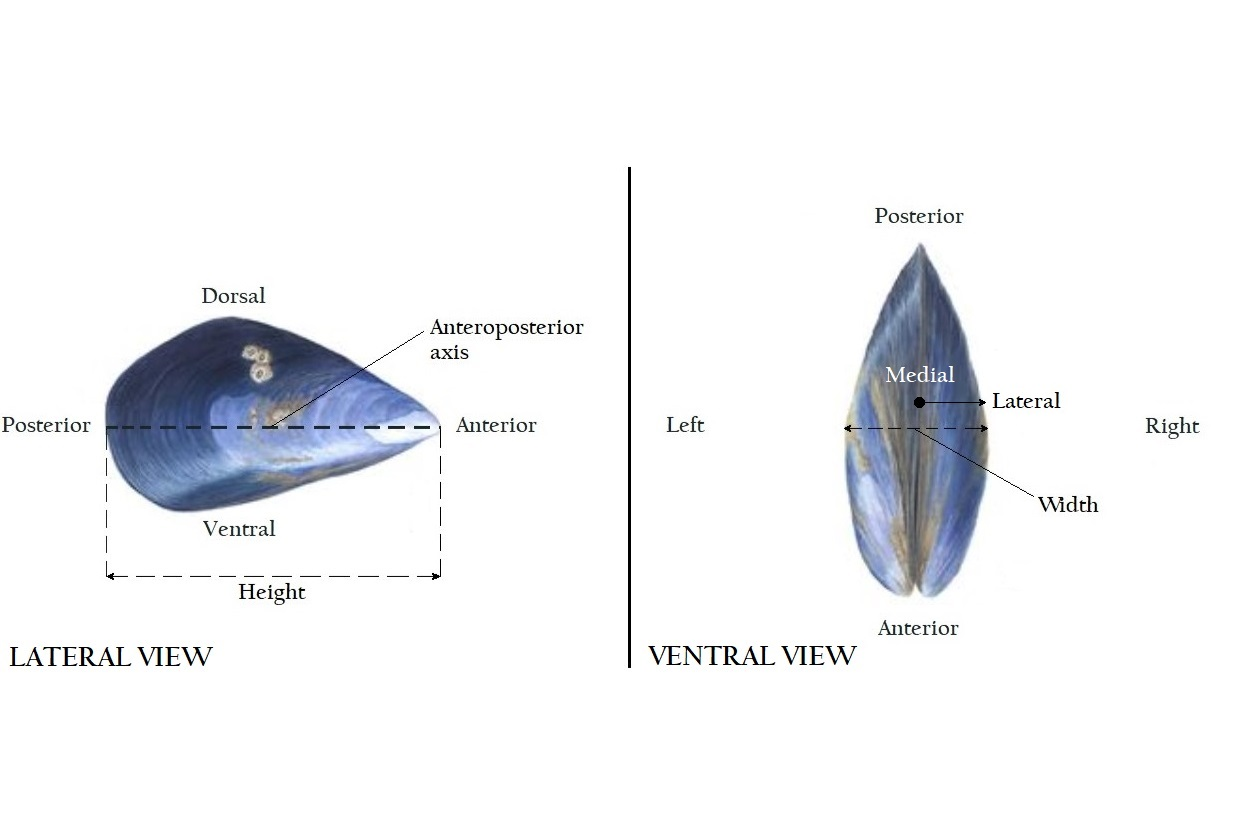
\includegraphics[width=\textwidth]{figures/Anatomy/M_edulis_anatomical_axis_lateral.jpg}
    \caption{The figure caption depends on if it ends up here, or in the material and method. Write when decided. The illustration was adapted from an artistic work by Abby Towne, A. Towne Design with permission.}
    \label{fig:anatomical_axis}
\end{figure}


\subsection{Classification of the haemocyte subpopulations of \emph{M. edulis}}
\label{subsection:haemocyte_classification}
Since the first written account on the subject (\cite{Cuenot1891}, cited in: \cite{Cheng1980}), several authors have devoted their attentions to developing a unifying classification system for the amoebocytic blood cells of bivalve mollusks, more commonly known as haemocytes (\cite{Cheng1980, delaBallina2022}). Belonging to the bivalve familiy \emph{Mytilidae}, the haemocytes of \emph{Mytilus edulis}, \emph{Mytilus galloprovincialis} and several other commercially important species of the genus \emph{Mytilus} have been encompassed by these efforts, creating a substantial pool of literature on the haemocytes of this genus alone. Despite a lack of consensus for any unifying classification system for the haemocytes of this phylum at large, the literature that exists on the haemocytes of \emph{M. edulis} generally agrees on the existence of three distinct subpopulations.

The first effort to classify the haemocytes of \emph{M. edulis} was made by Moore and Lowe (1977). Much like the other attempts to classify bivalve haemocytes at the time, this classification was based on the morphofunctional aspects of these cells - a system that has been extensively reviewed by Hine (1999). Moore and Lowe constructed a simple classification based on static morphological and ultrastructural characteristics of the haemocytes, combined with their phagocytic capacities (\cite{Moore1977}). From routine cytological staining, they identified three haemocyte subpopulations (or cell types): "(1) small basophilic hyaline cells or lymphocytes, (2) larger basophilic hemocytes with varying degrees of irregular cytoplasmic granulation and vacuolation, and (3) eosinophilic granular haemocytes or granulocytes" (\cite{Moore1977}). The small basophilic cells (4-6 \micro m) were generally spherical in outline, had a scant thin rim of basophilic hyaline (read: transparent) cytoplasm and a spherical nucleus - bearing resemblance to vertebrate lymphocytes. The larger granular basophils (7-10 \micro m) displayed less intense basophilic cytoplasm, lower nuclear:cytoplasmic (N:C) ratios and more irregularly shaped nuclei. The eosinophilic granulocytes were the largest cell type identified (7-12 \micro m). They had a regular spherical appearance, further characterized by a small round nucleus, low N:C ratio, and a cytoplasm filled with spherical eosinophilic granules (0.5-1.0 \micro m).

Electron micrographs confirmed the existence of three ultrastructurally distinct morphologies. Except for a few mitochondria, the lymphocyte-like cells contained a scarcity of organelles and granules. This stood in sharp contrast to the larger granular basophils, which contained Golgi apparatus, phagosomes and smaller granular inclusions - possibly representing primary lysosomes. A phagocytosis assay with experimentally injected carbon particles revealed that both granular cell types displayed phagocytic properties, while the small lymphocyte-like cells did not show any evidence for this capacity. To reflect this functional evidence, the granular basophilic haemocytes were classified as phagocytic macrophages. (\cite{Moore1977})

The morphological and ultrastructural findings of Moore and Lowe (1977) have since been confirmed by several investigators (\cite{Rasmussen1985, Renwartz1990, Pipe1990, Noel1994, Pipe1997, Wootton2003}). From their stand-alone electron microscopical examinations, Pipe and colleagues (1990) made a distinction between granular haemocytes with small (0.2-0.3 \micro m) and large (0.5-1.5 \micro m) granules. By relating the two ultrastructural phenotypes to their cytological staining properties, investigators soon demonstrated that the two cell types corresponded to the basophilic and eosinophilic granular haemocytes of Moore and Lowe (\cite{Pipe1990, Noel1994}). Thus, if reduced to it's static morphological criteria, Moore and Lowe's classification of \emph{M. edulis} haemocytes coincides with the original system of Cúenot (1891). This system generally recognized three types of haemocytes in bivalves: "(1) finely granular haemocytes, (2) coarsely granular haemocytes and (3) cells with very little cytoplasm surrounding the nucleus" (\cite{Cheng1984}). 

Leaning towards a phylum-wide two-categorical classification (hyalinocytes and granulocytes), Cheng (1981) argued that a distinction between the basophillic and eosinophilic granulocytes of \emph{M. edulis} was artificial, as he saw them as being immature and mature stages of the same cell type (granulocytes), respectively. From observations of what resembled intermediate stages between the lymphocyte-like and larger basophilic cells, Moore and Lowe (1977) had argued that the basophilic cells constituted an ontogenic developmental series, with the larger phagocytic macrophages representing the final stage of differentiation. This was further supported by observations of lymphocyte-like cells with mitotic figures, suggesting that it could be the stem cell of this lineage (\cite{Moore1977}). Since a few smaller eosinophilic granulocytes (5-7 \micro m) were observed in their sections, the eosinophilic granulocytes were believed to represent a distinct growth series.

As noted by Cheng (1984), this theory was not based on direct evidence, but consisted mainly of interpretive evaluations of morphological findings. The classification of bivalve haemocytes should ideally be constructed on the basis of their ontogeny. However, mapping of ontogenic lineages has been tempered by the lack availible molecular databases, no one unifying model species, combined with uncertainty regarding the hematompoietic tissue(s) and processes of bivalves (\cite{Hine1999, Smith2016, Pila2016, delaBallina2022}). With no real ontogenic evidence to work with, a careful assessment of the availible morphological data may represent a better alternative than founding the classification solely on biochemistry and function (\cite{Hine1999}). 

Almost two decades after flow cytometers became commercially availible in the 1970s (\cite{Shapiro2004}), the application of these instruments started to gain traction within the field of invertebrate immunopathology (\cite{Fisher1988}). Since the traditional characterization of bivalve haemocytes was largely based on morphological criteria such as size, granularity and staining affinities, the simultaneous measurement of forward scatter (\acrshort{fsc}, $\approx$ size) and side scatter (\acrshort{ssc}, internal complexity $\approx$ granularity) represented a far less subjective approach to their characterization (\cite{AshtonAlcox1998, Allam2002, Mateo2009}).

A detailed flow cytometric characterization of the haemocytes of \emph{M. edulis} was undertaken by Le Foll and colleagues (2010), who were able to distinguish three subpopulations according to their cell diameters (\micro m) and Side Scatter (\acrshort{ssc}) (\cite{LeFoll2010}). These comprised one population of small cells (7.14$\pm{0.05}$ \micro m) with low \acrshort{ssc}, one population of larger cells (9.97$\pm{0.17}$ \micro m) with intermediate \acrshort{ssc} and one population of large cells (10.08$\pm{0.24}$ \micro m) with high \acrshort{ssc}. By running haemocytes stained with eosin - which is fluorescent in the green/yellow spectrum under blue laser exitation (\cite{Elfer2016, Koegle2020}) - they were able to identify the latter cluster as eosinophilic granulocytes. The use of flow cytometers equipped with cell sorting capabilities simplifies the process of verifying any classification derived from flow cytometric measurements (\cite{Shapiro2004}). However, when extracting cells with known measured characteristics is not possible, the cells to be classified can be separated by other means prior to flow cytometric acquisition.

Realizing that the three cell types of \emph{M. edulis} differed with regard to the size and density of their granules (or the lack thereof), Friebel (1995) and Pipe (1997) managed to physically separate the eosinophilic granulocytes from the two basophilic cell types by density centrifugation (\cite{Friebel1995, Pipe1997}). Dependent on the treatment prior to centrifugation (fixative, staining), this generally resulted in a separation of the whole haemocyte population into three distinct cell-bands. The two basophillic cell types could be isolated from the upper cell band (lowest density), the eosinophilic granulocytes from the lower, while the intermediate fraction often consisted of varying proportions of all three cell types. Accompanied by the rapid growth of flow cytometric applications in invertebrate immunology, the progress made by Friebel (1995) and Pipe (1997) meant that results from functional and biochemical assays could be assigned to specific cell types at a higher throughput. Thus, the unraveling of the roles of individual haemocyte subpopulations really started to pick up speed.

\section{The role of hemocytes}
Functional classification based on phagocytic capacity: Differences in phagocytosis between granulocytes and agranular haemocytes may be related to the type of phagocytosed particles involved, rather than differences in phagocytic ability (Hine, 1999)


Unlike granulocytes and hyalinocytes, precursor cells do not contribute to immune-response mechanisms such as phagocytosis or encapsulation, and they also lack common intracellular enzyme systems associated with host defence. 

Their lack of cytoplasmic organelles seems to preclude a secretory or phagocytic function

Basophilic cytoplasm suggest the presence of free ribosomes and immaturity

Refer to the 1990 study of Pipe when explaining the functions of the cytoplasmic granules.


Hemocytes also (in addition to lung and digestive gland) showed high expression levels (of initiator and executioner caspases), probably due to the role of apoptosis in the defense against pathogens. Because bivalves are highly susceptible to climate changes, pollutants and pathogens, it  could be suggested that a strong apoptotic process may be necessary to ensure body homeostasis. (Romero, 2011). See page 11 of (New Insights into the Apoptotic Process in Mollusks: Characterization of Caspase Genes in Mytilus galloprovincialis) for greater detail and references.

\section{Bivalve hemocytes as \emph{in vivo} and \emph{in vitro} model systems}
Used as membrane integrity model system. "Since their membranes are susceptible to being destabilised by different stressors, this feature has been frequently used as a biomarker to monitor pollution and animal health (reviewed in Moore et al. 2004, 2006)." From "Changes induced by two strains of Vibrio splendidus in haemocyte subpopulations of Mya arenaria, detected by flow cytometry with LysoTracker" (Mateo, 2009), DOI: 10.3354/dao02121 

Introduce ToPro-3, Calcein AM (Calcein acetoxymethyl) and \acrshort{apo15} (\cite{Barth2020}) and their principle of staining, i.e., dye exclusion, cell-permeable (non-specific esterase substrate) and binding to phosphatidyl serine externalized during programmed cell death.

\acrshort{calceinam} is an electrically neutral molecule, which can easily penetrate cells through diffusion. After acetoxymethyl ester hydrolysis, the negatively charged Calcein molecules are trapped within the cell.

Theory behind Annexin-V/Apo-15: Annexin V
has affinity for phosphatidylserine, which is externalized to the
outer layer of the plasma membrane in the earlier stages of apoptosis. Annexin V also binds internal phosphatidylserine in permeable membranes, i.e. dead cells. Thus, dead cells are Apo-15+ ToPro3+, while the early apoptotic cells are only Apo15+.

The total hemocyte count (\acrshort{thc}) decreased by 66\% after a bacterial injection \cite{Parisi2008}. This could actually be to hemocyte aggregation in response to the needle injection itself.
\chapter{Material and method}
\label{chap:m&m}

\section{Material}
\subsection{Laboratory instruments}
\begin{table}[H]
	\centering
	%\caption{Chemicals used in the master thesis, listed alphabetically according to chemical name, including the chemical's CAS nr., purity/grade, supplier and state.}
	\label{tb:instruments}
	\resizebox{\linewidth}{!}{
	\begin{tabular}{lll}
	\textbf{Instrument} & \textbf{Model} & \textbf{Producer} \\
		\midrule
   Benchtop Flow Cytometer               & BD Accuri$^{TM}$ C6 Plus & BD Biosciences, California, US \\
   Submersible Flow Cytometer            & Cytosub                  & CytoBuoy, Woerden, NL \\
   Coulter Counter                       & Multisizer 4             & Beckman Coulter Inc., California, US \\
   Upright microscope                    & Eclipse Ni-U             & Nikon Corp, Tokyo, JP \\
   Upright microscope                    & Ecliplse 90i             & Nikon Corp, Tokyo, JP\\
   Transmitted/incident light microscope & Labrolux 12              & Leitz, Wetzlar, DE\\
   Benchtop centrifuge                   & Centrifuge 5804 R        & Eppendorf, Hamburg, DE\\
   Counting chamber                      & Bürker                   & Hirschmann-Laborgeräte, Eberstadt, DE \\
   		\bottomrule
	\end{tabular}
}
\end{table}



\subsection{Chemicals}
\begin{table}[H]
	\centering
	%\caption{Chemicals used in the master thesis, listed alphabetically according to chemical name, including the chemical's CAS nr., purity/grade, supplier and state.}
	\label{tb:chemical-list}
	\resizebox{\linewidth}{!}{
	\begin{tabular}{lllll}
	\textbf{Chemicals (abbrv.)} & \textbf{CAS-No.} & \textbf{Purity/grade} & \textbf{Supplier} & \textbf{state} \\
		\midrule
    Calcium chloride dihydrate      & 10035-04-8 & $\geq$ 99.0 \% & Sigma Aldrich & s \\
    Dimethyl sulfoxide              & 67-68-5    & $\geq$ 99.5 \% & Sigma Aldrich & l \\
    D-(+)-Glucose                   & 50-99-7    & $\geq$ 99.5    & Sigma Aldrich & s \\
    \ce{Na2EDTA}$\cdot$\ce{2H2O}    & 6381-92-6  & 98.5-101.5 \%  & Sigma Aldrich & s \\
    Ethanol                         & 64-17-5    & 96 \% vol      & VWR           & l \\
    \ce{Na2HPO4}$\cdot$\ce{2H2O}    & 10028-24-7 & $\geq$ 98.0    & Sigma Aldrich & s \\
    Potassium phosphate monobasic   & 7778-77-0  & $\geq$ 98.0    & Sigma Aldrich & s \\
    Copper(II)sulfate pentahydrate  & 7758-99-8  & $\geq$ 98.0    & Sigma Aldrich & s \\
    Formaldehyde                    & 50-00-0    & 37\% wt        & Sigma Aldrich & l \\
    HEPES                           & 7365-45-9  & $\geq$ 99.5 \% & Sigma Aldrich & s \\
    Magnesium sulfate heptahydrate  & 10034-99-8 & $\geq$ 99.5 \% & Sigma Aldrich & s \\
    Methanol                        & 67-56-1    & $\geq$ 99.9 \% & Sigma Aldrich & l \\
    Potassium chloride              & 7447-40-7  & $\geq$ 99.9 \% & Sigma Aldrich & s \\
    Sodium chloride                 & 7647-14-5  & $\geq$ 99.5 \% & Merck         & s \\
    Trizma\textsuperscript{\textregistered}base & 77-86-1    & ACS reagent    & Merck         & s \\
    TRIS HCl                        & 1185-53-1  & $\geq$ 99.0 \% & Sigma Aldrich & s \\
		\bottomrule
	\end{tabular}
	}
\end{table}


\subsection{Reagents for Flow Cytometry}
\begin{table}[H]
	\centering
	%\caption{Reagents and kits used in the master thesis, listed alphabetically according to product name, including manufacturer, supplier and supplier's catalogue number.}
	\label{tb:reagent-list}
	\resizebox{\linewidth}{!}{
	\begin{tabular}{lllll}
	\textbf{Product name (abbrv.)} & \textbf{Manufacturer} & \textbf{Supplier} & \textbf{Catalogue} & \textbf{Concentration} \\
		\midrule
    TO-PRO$^{TM}$-3 Iodide (642/661) &  InVitrogen$^{TM}$  & Thermo Fisher & T3605 & 1.2 \micro M \\
    Ethidium Homodimer-1 &  InVitrogen$^{TM}$ & Thermo Fisher &  E1169 & 4 \micro L/sample \\
    Apotracker$^{TM}$ Green & BioLegend & Fisher Scientific & 50-207-9934 & 560 nM \\
    Calcein-AM & Invitrogen$^{TM}$ & Thermo Fisher & C1430 & 170 nM \\ 
    CS\&T RUO beads & BD Biosciences & BD Biosciences & 661414 &  4 drops/mL \\
    8-peak validation beads & Spherotech & BD Biosciences & 653144 & 4 drops/mL \\
    6-peak validation beads & Spherotech & BD Biosciences & 653145 & 4 drops/mL \\
		\bottomrule
	\end{tabular}
	}
\end{table}


\subsection{Microscopy kits and reagents}
\begin{table}[H]
	\centering
	%\caption{Reagents and kits used in the master thesis, listed alphabetically according to product name, including manufacturer, supplier and supplier's catalogue number.}
	\label{tb:Microscopy-list}
	\resizebox{\linewidth}{!}{
	\begin{tabular}{llll}
	\textbf{Product name (abbrv.)} & \textbf{Producer} & \textbf{Supplier} & \textbf{Catalogue} \\
		\midrule
    Giemsa's azur eosin methylene blue solution & Merck & Sigma Aldrich & 1.09204.0500 \\
    Hemacolor\textsuperscript{\textregistered} & Sigma Aldrich & Sigma Aldrich & 1.11661 \\
    Eukitt\textsuperscript{\textregistered} Quick-hardening mounting medium & Orsatec GmbH & Sigma Aldrich & 03989 \\
    Type N Immersion Oil for Microscopy & Nikon & ? & MXA20234 \\
    Percoll$^{TM}$ & Cytiva Sweden AB & Sigma Aldrich & GE17-0891-02 \\
		\bottomrule
	\end{tabular}
	}
\end{table}

\subsection{Microscope equipment and software}
\begin{table}[H]
	\centering
	%\caption{Reagents and kits used in the master thesis, listed alphabetically according to product name, including manufacturer, supplier and supplier's catalogue number.}
	\label{tb:Microscope_software-list}
	\resizebox{\linewidth}{!}{
	\begin{tabular}{lll}
	\textbf{Equipment} & \textbf{Model} & \textbf{Producer} \\
		\midrule
   \multicolumn{3}{l}{\textbf{Setup for Nikon 90i:}} \\
   Microscope controller software           & iControl v.2.0.0.3        & Nikon Corp, Tokyo, JP \\          
   Light engine                             & EL6000                    & Leica Microsystems, Wetzlar, DE \\
   Microscope camera                        & DS-Fi1                    & Nikon Corp, Tokyo, JP\\
   DS-Fi1 camera controller                 & DS-U2                     & Nikon Corp, Tokyo, JP \\
   DS-Fi1 digital imaging software          & NIS Elements D v.3.22.15  & Nikon Corp, Tokyo, JP \\
   Microscope camera                        & DS-Fi1c                   & Nikon Corp, Tokyo, JP\\
   DS-Fi1c camera controller                & DS-U3                     & Nikon Corp, Tokyo, JP \\
   DS-Fi1c digital imaging software         & NIS-Elements F v.4.60     & Nikon Corp, Tokyo, JP \\
   Flat top microscope stage                & Proscan H101/2            & Prior Scientific, Cambridge, UK \\
   Microscope stage encoder                 & Lie5 1P N2KV              & Numerik Jena, Jena, GE \\
   Microscope stage controller              & Proscan II                & Prior Scientific, Cambridge, UK\\
   Filtercube                               & Brightline\textsuperscript{\textregistered} Led-Cy5-A  & Semrock \\
   Filtercube                               & B-2A                      & Nikon Corp, Tokyo, JP \\
   Stage micrometer cal. slide              & 2 mm, 0.01 mm interval    & Leitz, Wetzlar, DE \\
   Objective lens                           & Plan Apo 20X/0.75         & Nikon Corp, Tokyo, JP \\
   Objective lens                           & Plan Apo 60XA/1.40 Oil    & Nikon Corp, Tokyo, JP \\
   Objective lens                           & Plan Apo VC 100X/1.40 Oil & Nikon Corp, Tokyo, JP\\
   
   && \\
   \multicolumn{3}{l}{\textbf{Setup for Nikon Ni-U:}} \\
   Light engine                             & Sola SM II 365            & Lumencor Ink., Greenbrier, US \\
   CMOS camera                              & MC170HD                   & Leica Microsystems, Wetzlar, DE \\
   Microscope camera                        & 4KHDMI                    & DeltaPix, Smorum, DK\\
   Objective lens (Nikon Ni-U)              & Plan Fluor 40X/0.75       & Nikon Corp, Tokyo, JP \\
   Objective lens (Nikon Ni-U)              & Plan Fluor 100X/1.30      & Nikon Corp, Tokyo, JP \\
		\bottomrule
	\end{tabular}
	}
\end{table}




\subsection{Buffers and solutions}
\begin{table}[H]
	\centering
	\label{tb:buffers}
	\resizebox{\linewidth}{!}{
	\begin{tabular}{ll}
	\textbf{Buffer} & \textbf{Composition} \\
		\midrule
    MAS                   &  375.6 mM \ce{NaCl}, 28.97 mM Citric Acid$\cdot$3Na$\cdot$2\ce{H2O}, 113.8 mM D-Glucose, \\ 
                          & 2.6 mM Citric Acid$\cdot$\ce{H2O}, 11.5 mM \ce{Na2EDTA}$\cdot$\ce{2H2O}, pH=7.0, 0.2 \micro m filtered \\
    Anticoagulant buffer  & 55.5 mM D-glucose, 171.1 mM NaCl, 13.4 mM \ce{Na2EDTA}$\cdot$\ce{2H2O}, \\
                          & 0.05 M TRIS/HCl, pH=7.6, 0.2 \micro m filtered \\ 
    PBS                                  & 136.9 mM \ce{NaCl}, 2.7 mM \ce{KCl}, 10.1 mM \ce{Na2HPO4}, 1.8 mM \ce{KH2PO4} \\
    Sorensen Buffer       & 66.7 mM \ce{KH2PO4}, 66.7 mM \ce{Na2HPO4}$\cdot$\ce{2H2O}, pH=6.8, 0.2 \micro m filtered \\
    MPSS    &  470 mM \ce{NaCl}, 10 mM \ce{KCl}, 10 mM \ce{CaCl2}, 10 mM HEPES \\
                          & 47.7 mM \ce{MgSO4}, pH=7.41, 0.2 \micro m filtered \\
    Tris Buffered Saline  & 44.5 mM Trizma\textsuperscript{\textregistered}base, 5.5 mM TRIS-HCl, 450 mM \ce{NaCl}, pH=7.00 \\
		\bottomrule
	\end{tabular}
	}
\end{table}


\section{Method development}
This section describes in detail the work and experiments that were performed in the development of a hybrid flow cytometry- and microscopy-based version of The Mussel Micronucleus Cytome Assay by Bolognesi and Fenech (2012). The finalized assay is presented in it's entirety in the method section, in the context of it's application to test the potential genotoxic and cytotoxic effects of aged \ce{TiO2} and Ag engineered nanoparticles. The results from this section is presented in the Results chapter (\ref{section:Results_Method_Development}), and the reader can benefit from a read through that section before continuing with the method section and the main results (4.2).

\subsection{Haemolymph sampling technique}
To minimize the possibility of contaminating hemolymph samples during extraction, a simple and time-effective sampling technique adapted from the nonlethal technique of Gustafson et al., 2005 was used. "Blind" methods of withdrawal through a notch in the posterior dorsal shell or through the exhalant syphon frequently resulted in considerable contamination with debris from the pallial fluid. Therefore, the hemolymph sampling technique employed was centered around achieving good visual contact with the posterior adductor muscle and the position of the needle within the muscle during hemolymph withdrawal, and was mainly constricted by the requirement of an intact digestive gland.

The digestive gland is located dorsally (towards the hinge), slightly off-center towards the anterior end of the shell (Eggermont, 2020). In order to access and see the posterior adductor muscle while staying clear of the digestive gland, the valves were prised apart ventrally by gently forcing a tissue forceps between the valves midway of the mussel's length, or slightly posterior of the byssal mass (Fig. \ref{fig:Hemolymph_sampling_illustration}a). When the pallial cavity opened, pallial fluid (seawater) was drained away from the posterior adductor muscle by positioning the mussel's umbo on a paper tissue for 15-30 seconds. Since the posterior adductor muscle is oblong in the anteroposterior direction, penetrating the muscle from the posterior end pointing straight anteriorly gave the operator better margins to avoid piercing the muscle.

To create a free path to the muscle from the posterior direction, the connecting mantle immediately surrounding the exhalant syphon were cut with a scalpel (Fig. \ref{fig:Hemolymph_sampling_illustration}b and d), holding the blunt spine of the blade facing the posterior adductor muscle. Thus, when illuminating the pallial cavity from above with the ventral aspect facing upwards, the operator was able to supervise the position of the needle inside the posterior adductor muscle sinus through the slightly transparent muscle fibers, as seen in Fig. \ref{fig:Hemolymph_sampling_illustration}c.

\begin{figure}[H]
    \centering
    \begin{subfigure}[b]{.45\textwidth}
        \centering
        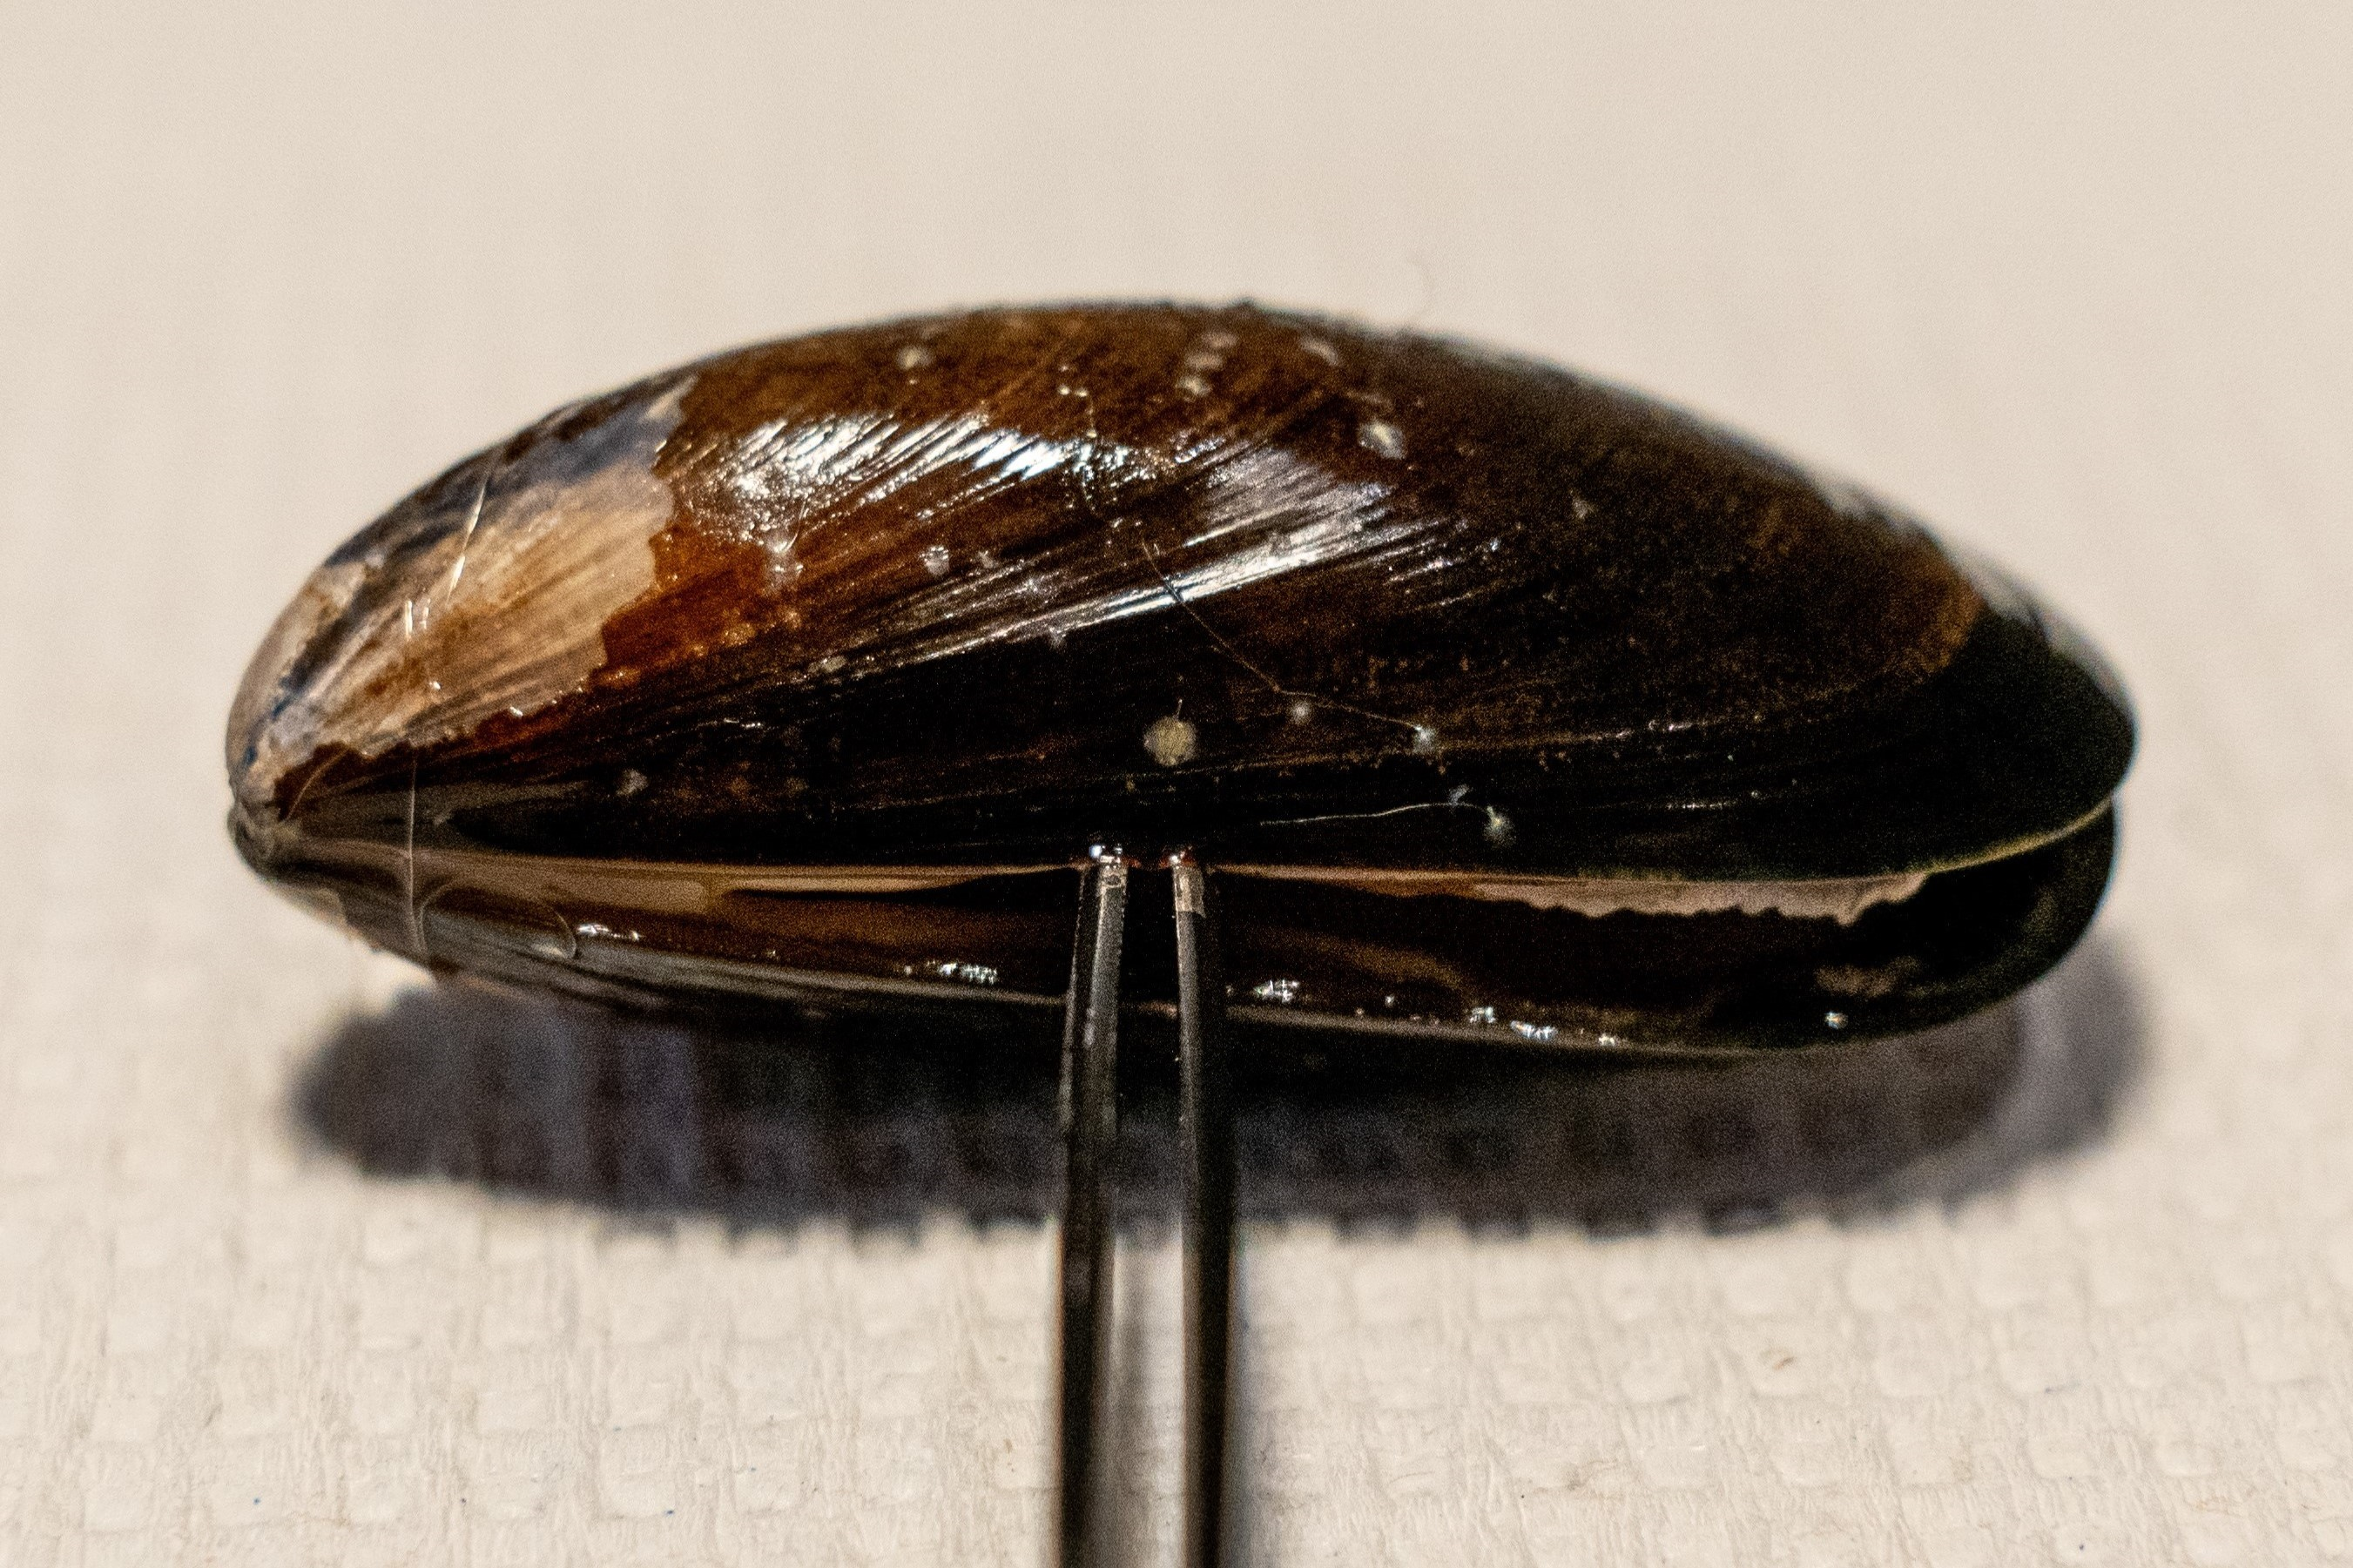
\includegraphics[width=\textwidth]{figures/Sampling technique/forceps square color.jpg}
        \caption{Placement of forceps between valves on the ventral side of the mussel.}
        \label{sfig:a}
    \end{subfigure}
    \hfill
    \begin{subfigure}[b]{.45\textwidth}
        \centering
        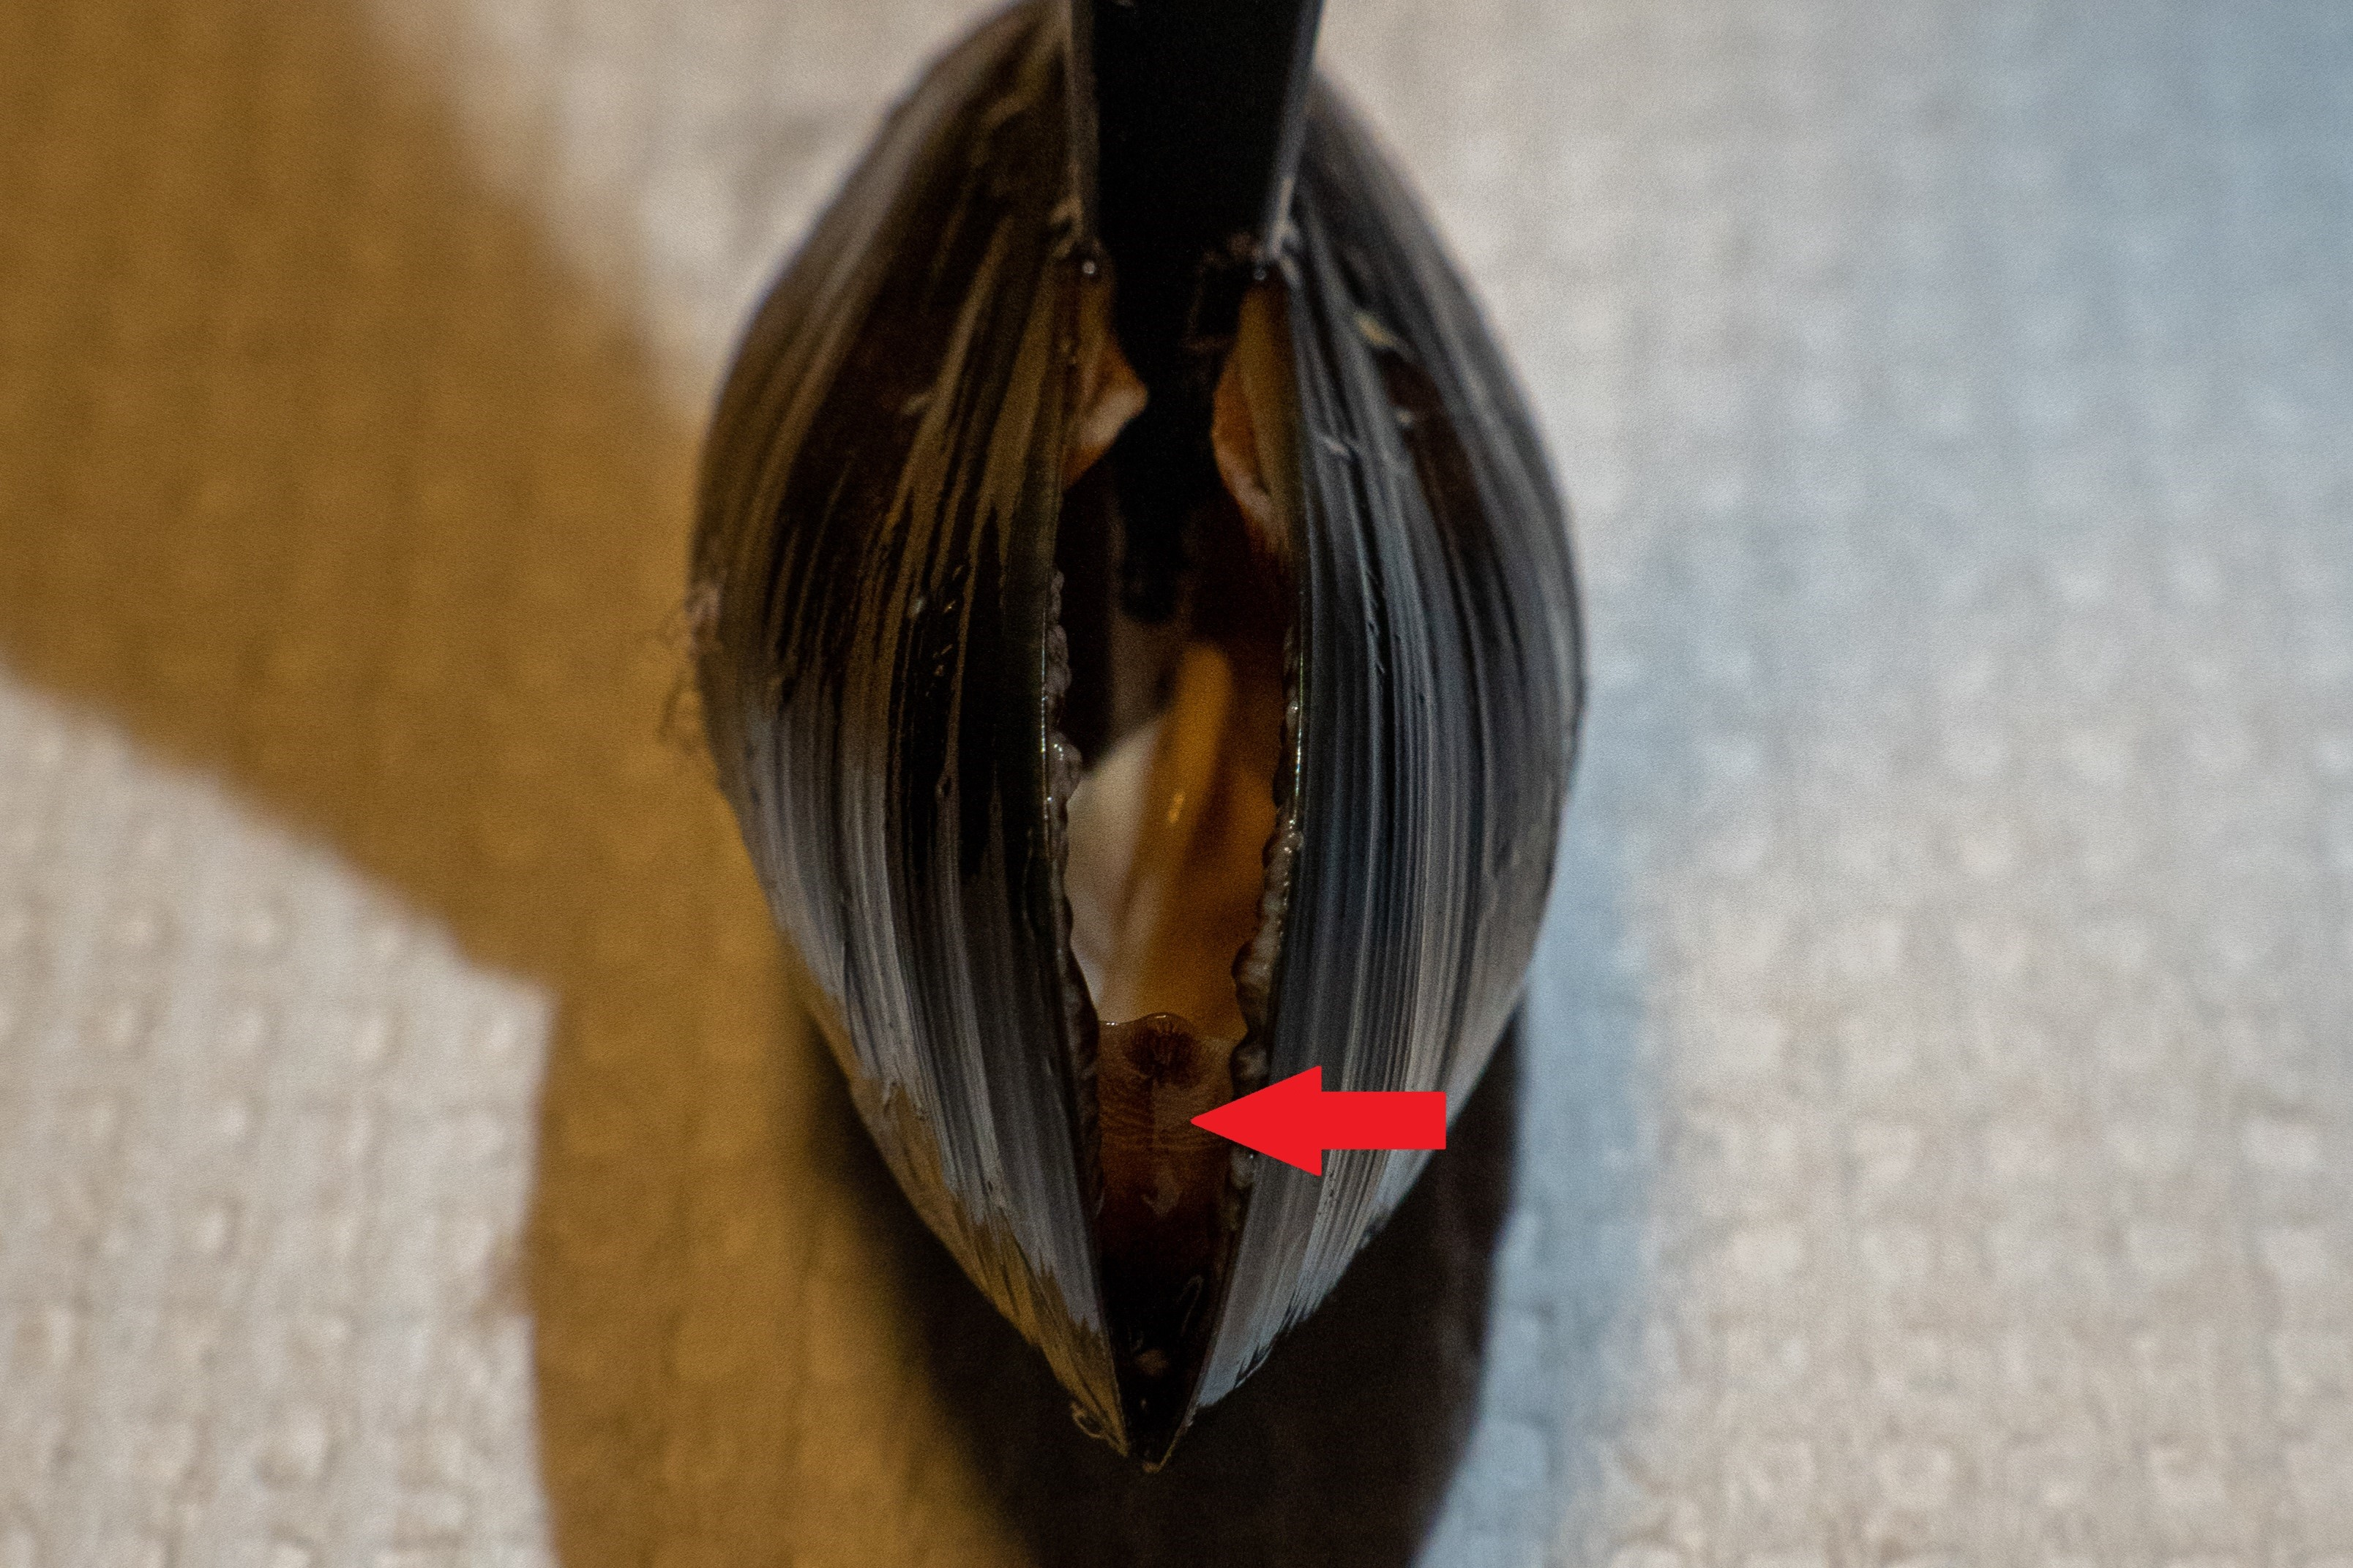
\includegraphics[width=\textwidth]{figures/Sampling technique/uncut color 3495.jpg}
        \caption{Posterior aspect of mussel with the connecting mantle (red arrow) intact.}
        \label{sfig:b}
    \end{subfigure}
    \newline
    \begin{subfigure}[b]{.45\textwidth}
        \centering
        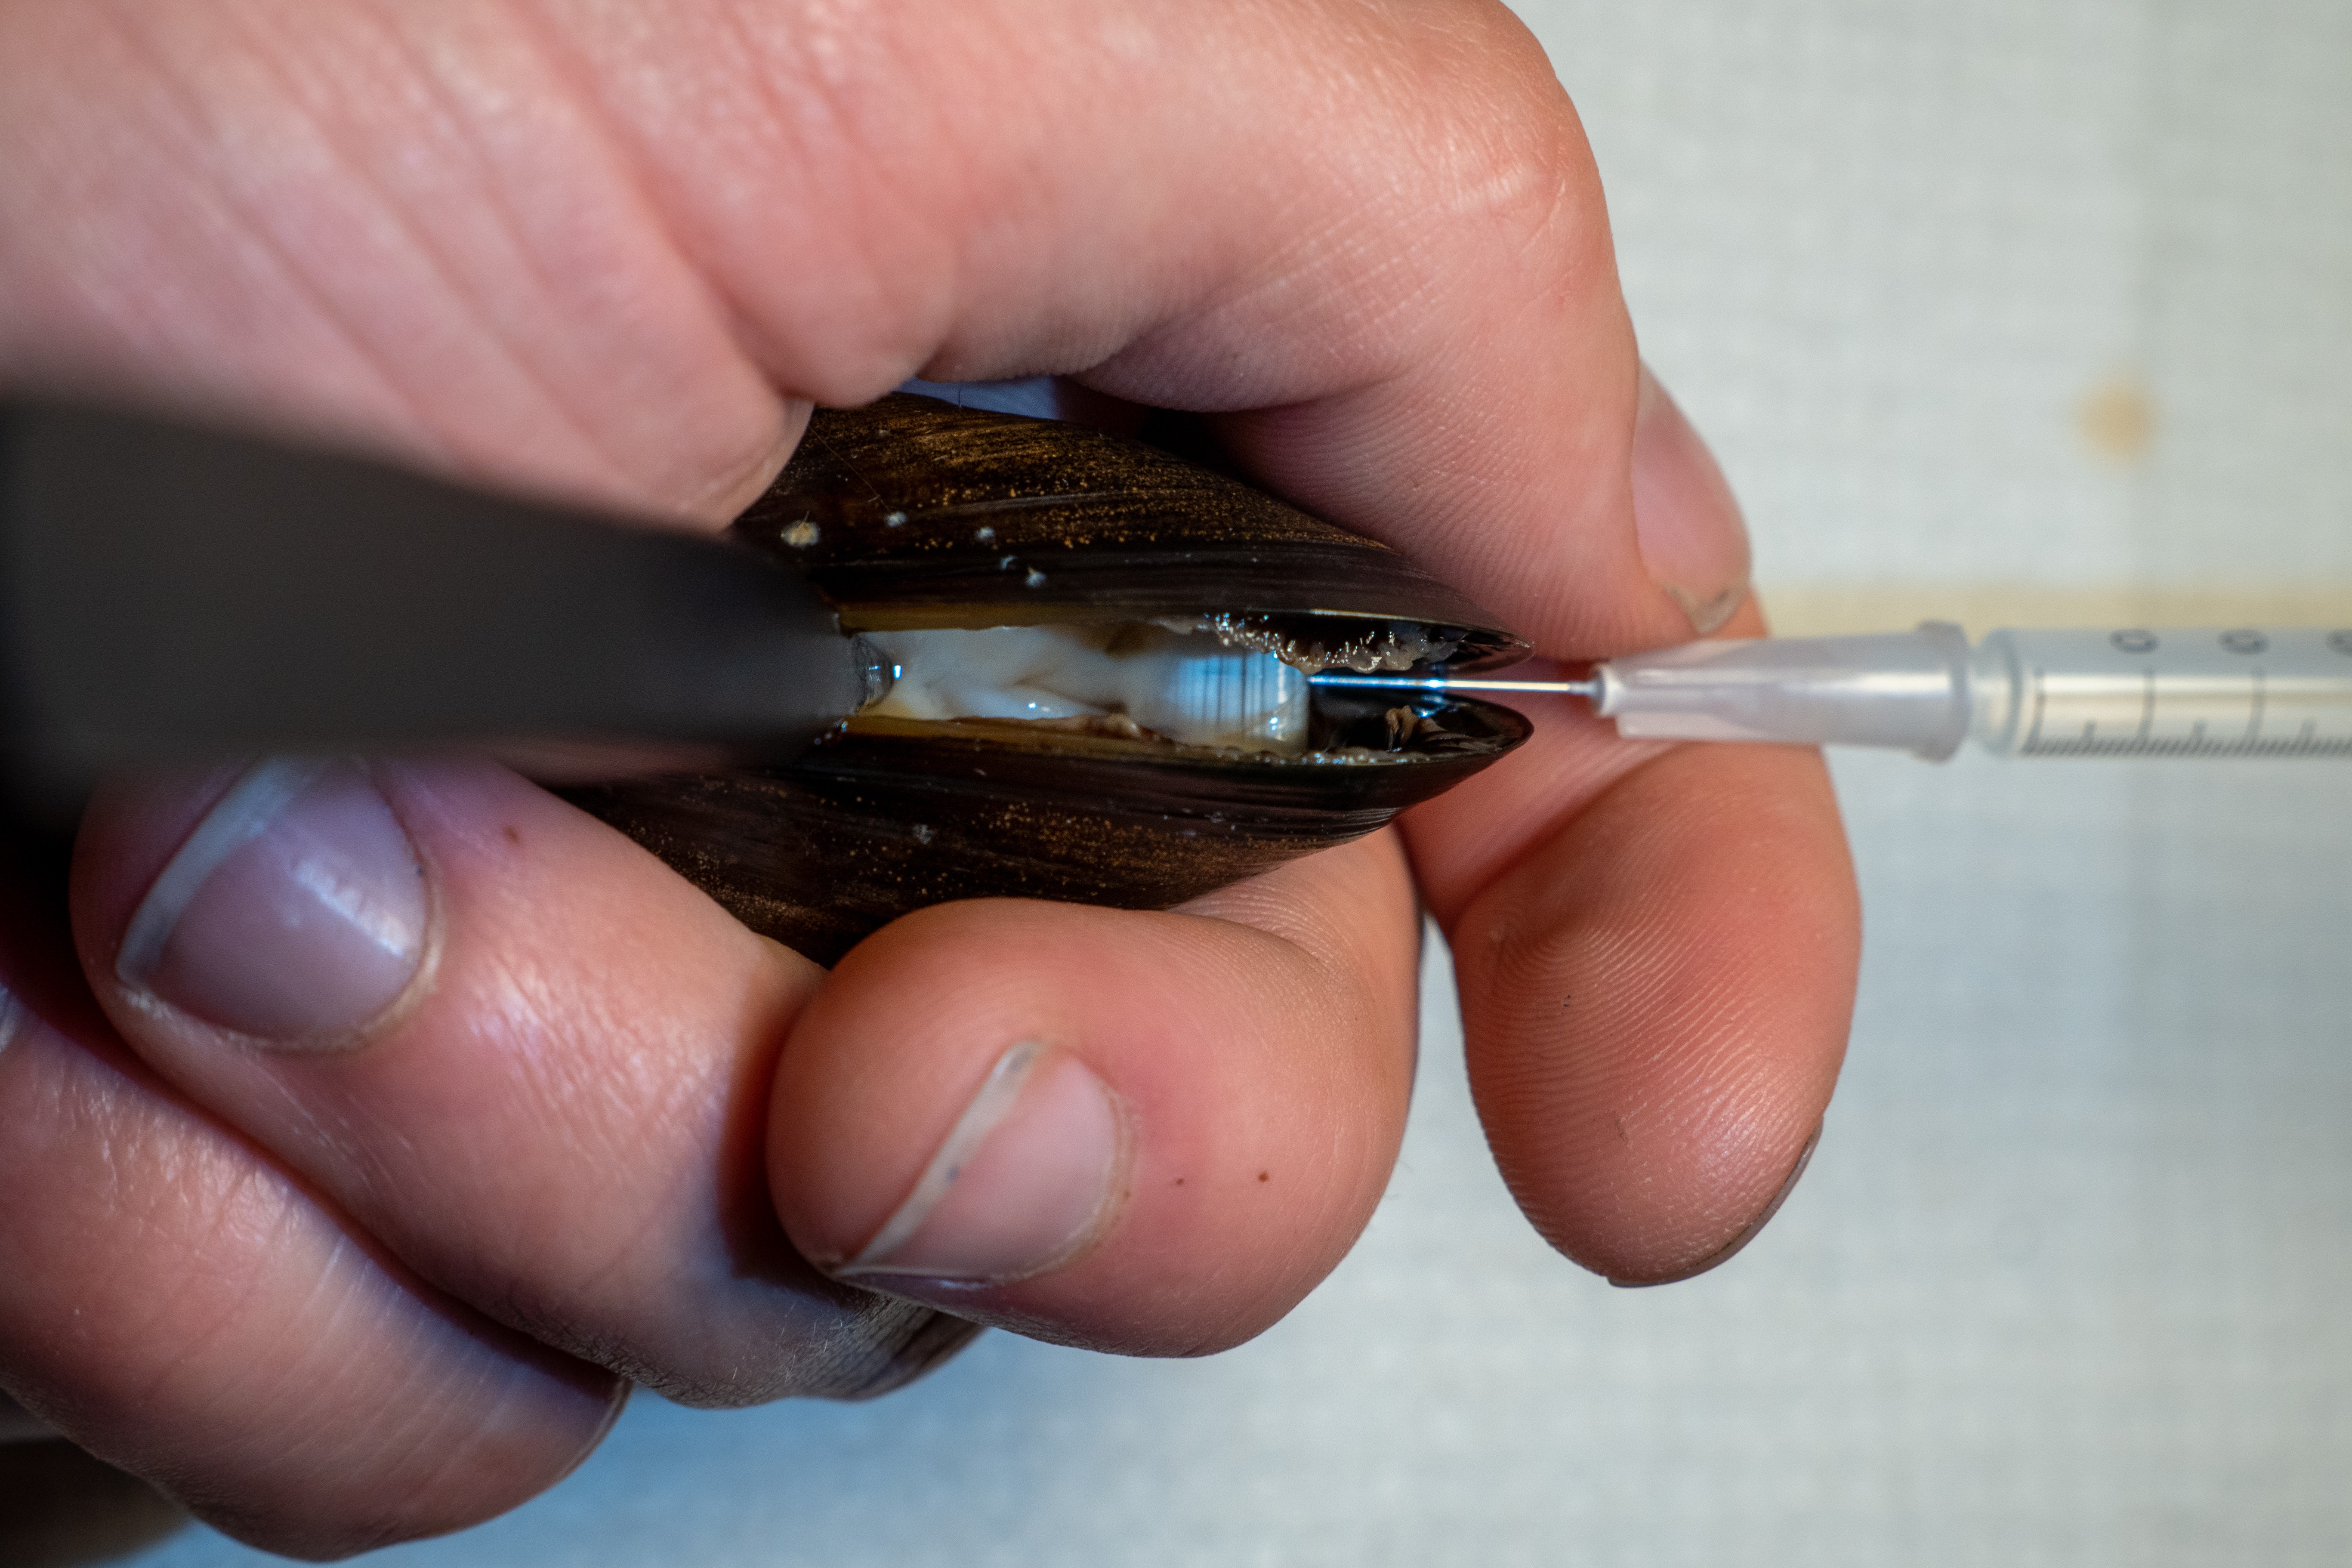
\includegraphics[width=\textwidth]{figures/Sampling technique/hands colors centered.jpg}
        \caption{The mussel grip and needle alignment employed, seen from the operators perspective.}
        \label{sfig:c}
    \end{subfigure}
    \hfill
    \begin{subfigure}[b]{.45\textwidth}
        \centering
        \includegraphics[width=\textwidth]{figures/Sampling technique/possible match.jpg}
        \caption{Mussel with visible posterior adductor muscle (red arrow) where the mantel was cut.}
        \label{sfig:d}
    \end{subfigure}
    \caption{An illustration of the method employed to extract hemolymph from the posterior adductor muscle of M. edulis in order to avoid off-target withdrawal of pallial fluid or spermatozoa. The images were captured using a Sony A6400 mirrorless digital camera with a Tamron 17-70mm F/2.8 lens, and were edited with Adobe\textsuperscript{\textregistered} Lightroom Classic 12.0 image editing software.}
    \label{fig:Hemolymph_sampling_illustration}
\end{figure}

For this work, 1.0 mL syringes equipped with sterile 23 gauge hypodermic needles were used. Hemolymph samples were gently withdrawn at an approximate rate of 1.0 mL/min, in order to prevent the negative pressure inside the muscle from drawing in pallial fluid between the muscle fibers. The mussels were placed in the palm of the operator's non-dominant arm, 3$^{rd}$-5$^{th}$ digits firmly gripping the mussel, 1$^{th}$ and 2$^{nd}$ digits keeping the syringe steady in the anteroposterior direction, while the dominant hand were used to withdraw the syringe plunger.

\subsection{Selection of haemocyte medium for flow cytometry assays}
The haemocytes of \emph{M. edulis} have a tendency to form aggregates upon mechanical stress, e.g. when the hemolymph is withdrawn through a thin syringe needle. Since accurate flow cytometric analyses rely on single-cell measurements, there was a need to minimize haemocyte aggregation during staining procedures, until the samples could by analyzed on the flow cytometer. In the literature, several authors have dealt with this challenge by aspirating hemolymph samples directly into slightly acidic EDTA-containing solutions buffered by citric acid (\cite{Söderhall1983, Bachere1988, LeFoll2010}). Since haemocyte aggregation is a Ca$^{2+}$-dependent process (\cite{Torreilles1999, Chen1995}), withdrawal of hemolymph into buffers containing divalent metal-ion chelators effectively slows the rate of haemocyte aggregation, allthough it does not inhibit aggregation completely (\cite{Chen1995}). Another frequently reported method is to dilute the hemolymph in cold filtered seawater (FSW), while keeping the samples on ice prior to analysis. 

In search for the most effective method for this work, hemolymph samples were withdrawn into syringes pre-filled with a number of different "anticoagulant" or "antiaggregative" buffers (1:1) reported in the literature. The degree of aggregation was initially evaluated by inspecting hemolymph smears prepared following the method of Bolognesi and Fenech (2012) under 10x magnification. After preliminary testing, the most promising buffers encountered where the Modified Alsever's Solution (MAS, pH=6.2), and the similar Anticoagulant Buffer (ACB, pH=7.6) with EDTA reported by \cite{Pipe1997}. Since the use of EDTA (MAS and ACB), acidic pH (MAS) or keeping samples on ice (FSW) might introduce inconveniences related to staining procedures, extra handling requirements and possibly impairing haemocyte viability, two experiments were devised in order to test their relative effects on haemocyte aggregation and viability - under the conditions intended for our flow cytometric analysis. Thereby, a cost-effect assessment could be carried out to arrive at the most suitable buffer for this work.

\subsubsection{Haemocyte aggregation}
An experiment was seeded from the observation that FCM singlet haemocyte counts tended to decrease over time from hemolymph withdrawal, and were based on the assumption that aggregation was the main driving factor. The proportion of aggregated haemocytes in a sample at a given time could therefore be retraced from the initial haemocyte count when performing several counts of the same sample over time. Since the difference in density between buffers would be negligible, the sedimentation rates would be independent of the haemocyte medium. Any observed differences would thus be caused by differences in the buffers' ability to inhibit aggregation.

500 \micro L hemolymph was withdrawn from 23 individual mussels into syringes prefilled with either 500 \micro L MAS (RT, n=7), ACB (RT, n=8) or cold Hemolymph Saline (MPSS, \SI{4}{\celsius}, n=8). Tris-buffered MPSS (pH=7.4) was used as a proxy for FSW, such that pH and osmolarity could be controlled. The diluted hemolymph was transferred to 12$\times$75 mm polystyrene tubes and the initial haemocyte count were determined by acquiring 20 \micro L sample on the flow cytometer immediately thereafter. Each sample was run with identical acquisition and fluidics settings (see table \ref{tb:FCM_settings}), and the cells were gated on by a singlet inclusion gate (FSC-A vs. FSC-H) and a haemocyte gate (FSC-A v. SSC-A, see gating strategy). To account for any extra aggregation occurring from gentle mixing with flow cytometry reagents in the planned assay, each sample was gently pipetted up and down four times following the initial count. The second count were performed precisely 15 minutes later to mimic the incubation periods of our flow cytometry reagents. Three more singlet haemocyte counts where acquired from each sample at 30, 45 and 60 minutes post-withdrawal, to discern the buffers' ability to prevent aggregation during longer incubation periods. Samples withdrawn into MPSS were kept on ice between each singlet haemocyte count.

\subsubsection{Logistic regression of the proportion of aggregated haemocytes}

The proportion of aggregated haemocytes where calculated according to equation \ref{eq: proportion_agg}.

\begin{equation}
    \label{eq: proportion_agg}
    \hat{p} = \dfrac{N_{t0} - N_{tx}}{(N_{t0} - N_{tx}) + N_{tx}} = \dfrac{N_{t0} - N_{tx}}{N_{t0}}
\end{equation}

\begin{equation}
    \label{eq:agg_free_matrix}
    y = 
    \begin{pmatrix}
      N_{t0_{1}} - N_{tx_{1}} &  N_{t0_{1}} \\
      N_{t0_{2}} - N_{tx_{2}} &  N_{t0_{2}} \\
      N_{t0_{3}} - N_{tx_{3}} &  N_{t0_{3}} \\
      \vdots                   & \vdots       \\
      N_{t0_{n}} - N_{tx_{n}} &  N_{t0_{n}} \\
    \end{pmatrix}
\end{equation}
\
Where $\hat{p}$ is the proportion of aggregated haemocytes, N$_{to}$ is the initial number of singlet haemocytes in the sample and N$_{tx}$ is the number of singlet haemocytes at time x after hemolymph withdrawal. The proportion of aggregated haemocytes were modelled as a function of log time, with buffer as a categorical explanatory variable, using the base R glm() function with a "quasibinomial" error distribution and "logit" link function, as shown in Code listing 3.1. Instead of using the calculated proportions ($\hat{p}$), the response variable was formatted as a two-column matrix of aggregated and singlet haemocyte counts (see equation \ref{eq:agg_free_matrix}), such that logistic regression was possible. The logistic GLM model coded the categorical explanatory variable's factor levels into dummy variables (see equation \ref{eq:dummy_variables}), and used the MAS buffer as reference level. The resultant logistic model can be written out as in equation \ref{eq:logit} on the original scale, where $\alpha + \beta_{1}x_{i}$ is the linear predictor of the reference level, $\alpha_{2}$ and $\alpha_{3}$ are the difference in y-intercept for the MPSS and ACB buffers, while $\beta_{2}$ and $\beta_{3}$ are the differences in slopes for the same buffers, respectively. The data is presented in figure \ref{fig:aggregation}, together with the three buffers' "sub-models".

\begin{lstlisting}[language=R, caption = {The R source code run to fit the logistic proportion aggregation model.}]
model = glm(y ~ log(t) + Buffer + log(t):Buffer,
family = quasibinomial(link = "logit")
\end{lstlisting}

\begin{equation}
    \label{eq:dummy_variables}
D_{2} =\begin{cases}
      1, & \text{MPSS}\\
      0, & \text{not MPSS},
    \end{cases}
    \quad
D_{3} =\begin{cases}
      1, & \text{ACB}\\
      0, & \text{not ACB}
    \end{cases}
\end{equation}

\begin{equation}
\label{eq:logit}
\hat{p}_{i} = \dfrac{1}{1 + e^{-(\alpha \: + \: \beta_{1} x_{i} \: + \: \alpha_{2} D_{2} \: + \: \alpha_{3} D_{3} \: + \: \beta_{2} D_{2} \: + \: \beta_{3} D_{3} \: + \: \epsilon_{i})}}
\end{equation}

\subsubsection{Haemocyte viability}
One of the aims of this project was to count the number of necrotic haemocytes present in the hemolymph of \emph{M. edulis} by means of flow cytometry. Since the mussels were to be exposed to \ce{TiO2} and Ag nanoparticles \emph{in vivo} for 21 days, the targeted endpoint would be the number of necrotic haemocytes circulating in their hemolymph at the timepoint just before hemolymph extraction on day 22. Any acute effects on viability arising from the hemolymph extraction itself, or during incubation with the viability stains between extraction and count, would serve to obscure the potential \emph{in vivo} effect of the nanoparticles. When choosing a suitable anticoagulant buffer for the purpose of this measurement, is was therefore essential to make sure that the buffer itself did not interfere with the targeted endpoint.

To test wether the EDTA-containing buffers had any effects on haemocyte viability in the 15 minute time window required for staining, 500 \micro L hemolymph was withdrawn from 24 individual mussels into syringes prefilled with either 500 \micro L MAS (n=8) or ACB (n=8). Hemolymph from the last eight mussels were withdrawn into cold MPSS and kept on ice as negative EDTA-controls. The diluted hemolymph were transferred to 12$\times$75 mm polystyrene tubes, were they were stored for 15 minutes before staining 300 \micro L subsamples with 1.0 \micro L Calcein AM (50 \micro M) and 3.6 \micro L TO-PRO$^{TM}$-3 Iodide (100 \micro M) dissolved in DMSO. The samples were incubated in darkness for 15 minutes, before 10.000 haemocyte events were recorded on the flow cytometer without washing.

488 nm-exited green fluorescence from hydrolyzed Calcein were recorded on the FL1 detector with a 533/15 nm filter, while the 640 nm-exited far red fluorescence from DNA-bound TO-PRO$^{TM}$-3 Iodide were recorded on the FL4 detector with a 675/25 nm filter. The events were gated according to the gating strategy in figure (ref figure), obtaining counts of live (Calcein$^{+}$ToPro3$^{-}$), necrotic (Calcein$^{-}$ToPro3$^{+}$) and doubly stained (Calcein$^{+}$ToPro3$^{+}$) haemocytes, as well as non-cellular particles (Calcein$^{-}$ToPro3$^{-}$) and a total count. In this particular experiment the doubly stained haemocytes were counted as necrotic, as newly damaged or lysed haemocytes might still retain a degree of non-specific esterase activity. Hence, the percentage of necrotic haemocytes were calculated according to equation \ref{eq:necrotic hemocytes}.

\begin{equation}
    \label{eq:necrotic hemocytes}
    \text{Necrotic haemocytes (\%)} = \dfrac{n_{Calcein^{-}ToPro3^{+}} + n_{Calcein^{+}ToPro3^{+}}}{n_{total} - n_{Calcein^{-}ToPro3^{-}}} \times 100
\end{equation}

The 700 \micro L remaining of each hemolymph sample were stored for another 2 and 20 hours, and the same staining and flow cytometric measurements were repeated at these timepoints. Because of considerable aggregation and sedimentation of haemocytes in MPSS after 2 and 20 hours, and those kept in MAS and ACB for 20 hours, the haemocytes in these samples were resuspended with a wide bore pipette before the second and third rounds of staining.

\subsection{Cytologic characterization of M.edulis haemocyte subpopulations}
\label{subsection:morph}
For the purpose of characterizing and imaging the different haemocyte cell types of \emph{M. edulis} in a non-spread state, samples were withdrawn into an equal volume of ice-cold MPSS and transferred directly onto glass slides. The glass slides were kept in a humid chamber for up to 5 minutes before cells were fixed in ice cold methanol (5$\times$ 1 sec dips). This assured haemocyte attachment, but circumvented the profound morphological changes accompanied by the haemocytes’ process of spreading. Slides were stained with the Hemacolor\textsuperscript{\textregistered} kit according to the manufacturer’s recommendations, air dried, mounted with Eukitt\textsuperscript{\textregistered} and coverslipped. Stained haemocytes were examined and imaged under brightfield illumination on a Nikon Eclipse 90i upright microscope with a 100$\times$/1.40 oil immersion objective and a Nikon DS-Fi1 microscope camera.

Haemocyte morphology was primarily characterized on the basis of cytoplasmic staining, granularity (granule size, abundance and staining affinities), nuclear:cytoplasmic (N:C) ratio, size and shape. Since Le Foll and colleagues (2010) reported that the motile properties of the different haemocyte subpopulations of \emph{M. edulis} could be used as an additional functional criteria for their characterization, the spreading behavior of the different cell types were included to expand on the morphological characteristics. This comprehended a description of the typical haemocyte shapes and motile structures that were observable under differential interference contrast illumination in spread haemocytes. The preparation of slides with spread haemocytes followed a methodology similar to that of the non-spread haemocytes, but the humid chamber incubation periods prior to fixation and staining were extended (15-30 min). Microscopic fields were examined through a 60$\times$/1.40 oil immersion objective under DIC illumination.

\subsection{Determination of cell diameters}
\label{subsection:CytCar}
To establish wether haemocyte subpopulations differed with regard to size across a larger population of adult mussels, the cell diameters of 100 haemocytes were ascertained in haemolymph smears from 20 individual mussels (n=2000). Since the rate and degree of haemocyte spreading could be inherently different among cell types, all spreading was effectively impeded by collecting haemolymph samples into an equal volume of 5\% formaldehyde in MPSS. The fixation was continued for one hour in suspension, before cells were pelleted by centrifugation (250G, 15 min, \SI{10}{\celsius}) and resuspended in 100 \micro L 0.75 \% eosin in Sorensen Buffer. After staining for 5 minutes, 1 mL 3\% Wright’s-Giemsa was added and the staining was continued for an additional 15 minutes. Stained haemocytes were pelleted by centrifugation (180G, 12 min, \SI{10}{\celsius}), resuspended in 100-200 \micro L Sorensen Buffer and transferred onto glass slides. The slides were air-dried in a fume hood until the smears were completely dry and transparent, before they were mounted with Eukitt\textsuperscript{\textregistered} and coverslipped.

The slides were placed on the stage of a Nikon Eclipse 80i upright microscope, and 10-20 microscopic fields from each smear was photographed under DIC illumination with a $\times$60 oil immersion objective. Cell diameter measurements were performed digitally, using the \emph{Straight line tool} of the ImageJ image processing software (NIH, Bethesda, Maryland, US). The actual size of the magnified haemocytes were determined by calibrating the software's pixel/\micro m scale with a stage micrometer calibration slide (Leitz Wetzlar, Buffalo, DE), photographed with the same equipment and image resolution as the haemolymph smears. When haemocyte outlines deviated from an approximate spherical shape, the diameter was estimated as the average length of the long and short axes, after Burkhard et al. (2009). The measurements were performed as differential counts, such that the number of measurements of each cell type reflected their average relative proportions (\%) across all 20 mussels.

[Concider including measurements with the Coulter Counter as a comparison to cells fixed in formaldehyde. In that case, insert the methodology here.]

\subsection{Flow cytometric characterization of haemocyte subpopulations}
In order to


\subsubsection{Isopycnic centrifugation}
Formaldehyde-fixed haemocytes were separated on discontinuous Percoll gradients according to the protocol by Friebel and Renwrantz (1995), with minor modifications. The separation was performed in duplicate with pooled haemocytes from a total of six adult mussels (shell length 55-70 mm). For both gradients, the haemolymph of three individual mussels (1.5-2.0 mL/mussel) were withdrawn into an equal volume of 5\% formaldehyde in MPSS, wherein the haemocytes were fixed for one hour after pooling. The fixed haemocytes were stained with 0.75 \% Eosin and 3 \% Giemsa according to the procedure in section~\ref{subsection:CytCar}. After pelleting, stained haemocytes were resuspended in Tris-Buffered Saline (TBS, 900 mOsm) to an approximate concentration of $9\times10^{6}$ cells/mL, before layering 2 mL suspension on top of both gradients. Discontinuous Percoll gradients consisted of 15\%, 33\%, 38\%, 43\% and 90\% Percoll stock in TBS (vol/vol), and were constructed by carefully layering 2 mL of each Percoll concentration in 15 mL Falcon centrifuge tubes with conical bottoms (Corning, New York, US).

The centrifugation was started at 120G for 10 minutes (\SI{4}{\celsius}), followed by 40 minutes at 2500G. An Eppendorf 5804 R benchtop centrifuge equipped with an A-4-44 swing-bucket rotor was employed for the separation, with the brake ramp set to 1. The separated cell fractions were collected into syringes by puncturing the tubes below the gradient interfaces with 23G hypodermic needles. According to a protocol by Bachére and Grizel (1988), the Percoll was eliminated from the 43/90\% and 38/43\% fractions by two consecutive dilutions in TBS (1:7) and a 10\% sucrose cushions (1:1) before centrifugation (800G, 15 min, \SI{4}{\celsius}). Haemocytes collected from the 15/33\% interface were centrifuged directly after a seven-fold dilution in TBS (800G, 15 min, \SI{4}{\celsius}).

The pelleted cell fractions were resuspended in Sorensen buffer and divided into two aliquots; one aliquot were used to prepare smears according to the procedure in section \ref{subsection:CytCar}, while the remaining aliquots were further diluted in 1 mL Sorensen buffer for flow cytometric characterization. A total of 10.000 events were acquired from each cell fraction on the flow cytometer (36 \micro L flow rate, 16 \micro m core size), in addition to 30.000 events from both pools that were set aside prior to centrifugation. The relative proportion (\%) of cell types in each fraction were ascertained by performing 1000-cell differential counts.

\subsubsection{Identification of eosinophilic granulocytes by SSC and eosin fluorescence}
Since Eosin is fluorescent in the green/yellow spectrum (Ex$_{max}$/Em$_{max}$: 517/543 nm) (\cite{Koegle2020}), blue laser-exited fluorescence from this anionic dye can be collected on the FL1 detector (518-548 nm) of the BD Accuri C6 Plus flow cytometer (BD Biosciences, California, US). If the haemocytes of \emph{M. edulis} are permeabilized and stained with eosin prior to flow cytometric analysis, the fluorescent signal from Eosin can be used to identify eosinophilic granulocytes on FSC vs. SSC dotplots by backgating. This approach was attempted by Le Foll an colleagues (2010), who detached spread haemocytes stained by eosin with an EDTA/trypsin solution followed by flow cytometric analysis. As noted in the theory section (\ref{subsection:haemocyte_classification}), their results indicated that FL1$^{bright}$ events corresponded to haemocytes with high SSC values. However, this exact methodology did not result in two well-defined FL1$^{bright}$ and FL1$^{dim}$ peaks, such that the lower bound of their electronic FL1$^{bright}$ gate had to be drawn more or less arbitrarily. It could therefore not be used to quantify the proportion of eosinophilic haemocytes - especially since the identity of the FL1$^{bright}$ events were never verified by microscopy.

To investigate the potential application of eosin fluorescence and side scatter as discriminators in a flow cytometric differential count of \emph{M. edulis} haemocytes, an attempt to optimize the basic method of Le Foll et al. (2010) were undertaken. This process involved exploring different fixatives, methods of fixation, eosin staining solutions and the duration of both fixation and staining, in order to achieve a practically applicable resolution between eosinophilic granulocytes and the rest of the haemocytes.

Haemolymph was withdrawn from the posterior adductor muscle of 9 adult mussels into an equal volume of methanol (n=3), 3:1 methanol:glacial acetic acid (n=3) or 5\% formaldehyde in MPSS (n=3) and fixed for 30 minutes in suspension. The fixed haemocytes were pelleted by centrifugation (250G, 5 min, \SI{20}{\celsius}) and resuspended in the eosin component of the Hemacolor\textsuperscript{\textregistered} kit. After staining for 5, 10 or 15 minutes, the stained haemocytes were pelleted (180G, 5 min, \SI{20}{\celsius}), resuspended in 100 \micro L Sorensen buffer and transferred onto glass slides. The slides were coverslipped and inspected under brightfield illumination on a Nikon Eclipse Ni-U upright microscope with a 40x/0.75 objective.

The only smears without high degrees of unspecific binding were those fixed in 5\% formaldehyde. To reduce the passive diffusion of eosin into non-target cells, 5\% formaldehyde in MPSS was selected for further testing - being the softest fixative of the three. By diluting Eosin in Sorensen buffer, a set of staining solutions with 0.25\%, 0.5\%, 0.75\%, 1.0\%, 1.5\%, 3\%, 5\%, and 8\% Eosin (vol/vol) were prepared. The haemolymph of 4 new mussels where fixed in 5\% formaldehyde for 30 minutes, pooled and st 

\subsection{Scoring of necrotic haemocytes by flow cytometry}
To discriminate between viable and necrotic haemocytes by flow cytometry, a two-color fluorescence assay with the cell-permeant probe Calcein acetoxymethyl and the non-permeant dsDNA-binding dye TO-PRO$^{TM}$-3 Iodide (Molecular Probes, Eugene, OR) was chosen. This combination of probes was primarily selected for two reasons: (1) it enables simultaneous measurement of intracellular esterase activity and plasma membrane integrity - two recognized parameters of cell viability, and (2) there is virtually no fluorescent spillover between the probes, such that the uncompensated raw data can be used directly.

Since Calcein AM is commonly used in the LIVE/DEAD\textsuperscript{\textregistered} Viability/Cytotoxicity Kit for mammalian cells (Molecular Probes, Eugene, OR), the staining protocol of this kit was used as a guide for obtaining an adequate fluorescent signal from hydrolyzed Calcein on the FL1 detector (518-548 nm). The manufacturer's recommendation of 50 nM Calcein AM mL$^{-1}$ cell suspension (0.1-5 $\times 10^{6}$ cells) gave a bright fluorescent signal in live cells after 15 minute incubation, so no further optimization was required. Information on suitable concentrations of TO-PRO$^{TM}$-3 Iodide for flow cytometric dye exclusion tests was however sparse, such that this had to be determined experimentally.

\subsubsection{Determination of optimal TO-PRO$^{TM}$-3 Iodide staining concentration}
The optimal TO-PRO$^{TM}$-3 Iodide concentrations for a flow cytometric dye exclusion assay would ideally fulfill two requirements. The first would be to give the highest possible resolution between viable and necrotic cells in terms of fluorescent intensity. Secondly, and of equal importance; the concentration cannot be acutely cytotoxic to haemocytes within the time-frame of staining and flow cytometric acquisition. To determine a suitable range of concentrations for this assay, a pool of dead (70\% methanol 30 min) and freshly withdrawn haemocytes was prepared. The methanol-killed hameocytes were washed three times in MPSS, resuspended ACB and gently mixed with freshly withdrawn heamocytes in ACB. The suspension was divided into 11 aliquotes of 1 mL, and all but one was stained with TO-PRO$^{TM}$-3 in the range of 30 nM to 8 \micro M. After incubating for 15 minutes (protected from light), 10 000 events were acquired from each sample on the flow cytometer. To examine wether the fluorescent signal intensity increased with further incubation, the same samples were incubated for another 15 minutes before the measurement was repeated.

Red laser-exited fluorescence from dsDNA-bound TO-PRO$^{TM}$-3 Iodide was collected on the FL4 detector (675/25 nm) of the BD Accuri C6 Plus flow cytometer. A histogram representation of the fluorescence revealed two distinct populations of events: one population of ToPro3$^{-}$ events and one population of ToPro3$^{+}$ events. The mean fluorescent intensity (MFI) of the two populations were calculated for each aliquot, and the difference was plotted against the staining-concentrations of TO-PRO$^{TM}$-3 Iodide. In order to predict a suitable range of concentrations from the data, the MFI differences were regressed on the TO-PRO$^{TM}$-3 concentration using a log-logistic model. Since the data required a model range bound by 0 and some unknown positive integer (0, \emph{a}), a four-parameter log-logistic function from the remote drc() package was used (v3.0-1; \cite{drc}). This function allows the lower asymptote to be fixed to 0, as shown in code listing 3.2. The general function is seen in (\ref{eq:LL4}), where \emph{b} and \emph{e} represents the slope parameter and inflection point, while \emph{d} and \emph{c} represents the upper and lower asymptotes, respectively.

\begin{lstlisting}[language=R, caption = {The R source code run to fit the four-parameter log-logistic regression model in RStudio.}]
model = drm(y ~ x, data = df, fct = LL.4(fixed = c(NA, 0, NA, NA), 
names = c("b", "c", "d", "e")))
\end{lstlisting}

\begin{equation}
\label{eq:LL4}
y_{i} = c + \dfrac{d-c}{1 + (x_i / e)^b} + \epsilon_i
\end{equation}

Potential cytotoxicity at high concentrations was evaluated by examining the ToPro3$^{-}$ populations (SSC vs. FL4), to see wether any of the freshly withdrawn haemocytes were starting loose their ability to exclude TO-PRO$^{TM}$-3 Iodide.

\subsubsection{Gating Strategy}

\subsubsection{Method validation}




\section{Method}
\subsection{Animal housing}
Adult blue mussels (\emph{Mytilus edulis}) of x.x$\pm{5}$ cm shell length were obtained from Snadder og Snaskum AS (Indre Fosen, Norway). Upon arrival at the marine animal housing facilities of NTNU, Centre of Fisheries and Aquaculture (SeaLab), the mussels were transferred to 50 L filtered seawater flow-through tanks (11 L/min) supplied by a direct inlet from Trondheimsfjorden at 80 m depth ($\SI{7.5}{\celsius}$). Here, the mussels were kept to acclimatize for 2 days before transfer to the experimental exposure setup.

Time of mussel harvest/purchase?

Describe water treatment in more detail: include information regarding sand-filter, protein-skimmer, 0.5 um filter bags and UV-treatment.

Because the watertreatment left no natural feed for the mussels, the filtered seawater were supplemented with algae [insert species \& frequency].


\subsection{Experimental setup/design}
- Specs related to flowrate, feeding (alge conc: Coulter counter), how often was nano particles changed (every 3-4 days: check article), concentrations (ICP-MS --> mg/L in stocks and exp tanks), zetasizer --> size and surface potential

include figure of exp setup?

depuration period: check article

storage from depuration to sampling: mussels were not kept on ice, but were washed and taken directly upstairs for measuring weight, length, height and width for condition index, and were given to us for FCM sampling afterwards. If we were delayed, they were kept in the fridge until hemolymph sampling 

\subsection{Hybrid Micronucleus Assay}
Sampling
Flow Cytometer used and Flow Cytometry acquisition software
External software used for graphing and analysis of exported FCS files.
Replicate/triplicate measurements?
Number of events recorded for each mussel?
Briefly describe FCS and SSC.
Mention if data were collected in linear or logarithmic scale, 
FSC treshold (80.000 FSC-H). 
Fluorescent compensation (matrix)
Describe gating strategy herein? Debris exclusion (size); doublet exclusion --> haemocytes. (Gating of basophils and eosinophils, the use of FMO controls with TO-PRO-3 and/or the apoptosis stain) to create gates.

\begin{table}[H]
	\centering
	\caption{The FCM acquisition and fluidics settings specified with the BD Accuri C6 Plus acquisition software during the flow cytometric experiments reported in this work.}
	\label{tb:FCM_settings}
	\resizebox{\linewidth}{!}{
	\begin{tabular}{lllll}
	\textbf{Experiment nr.} & \textbf{Event-triggering threshold} & \textbf{Acquisition stop-condition} & \textbf{Flow rate (\micro L/min)} & \textbf{Core size (\micro m)} \\
		\midrule
    Aggregation & 80.000 FSC-H & acquired volume, 20 \micro L & 30 & 10 \\
    Calcein AM and TO-PRO$^{TM}$-3 Iodide & 80.000 FSC-H & 10.000 haemocyte events & 36 & 16 \\
    Apo-15 and TO-PRO$^{TM}$-3 Iodide & 80.000 FSC-H & 10.000 haemocyte events & 36 & 16 \\
		\bottomrule
	\end{tabular}
	}
\end{table}

\subsubsection{Scoring of necrotic haemocytes}

\subsubsection{Scoring of apoptotic haemocytes}

\subsubsection{Differential haemocyte count}

\subsubsection{Determination of haemocyte concentration}

\subsubsection{Slide preparation}
Refer to the MN cytome assay by Bolognesi, and mention that we fixed and stained haemocytes in suspension to produce slides without aggregated haemocytes. Since the cells were dead, they did not spread or produce pseudopodia, which allowed us to observe the actual size and form which they would posses ass they flowed through the laser of the flow cytometer.

\subsubsection{Scoring of MN and nuclear anomalies}

\subsubsection{Measurements and calculations}
(\cite{R-project})

\subsubsection{Statistical analysis}

\chapter{Results}
\label{chap:results}
\section{Identification of \emph{M. edulis} hemocyte subpopulations according to side scatter (SSC) and forward scatter (FSC)}
\subsection{Eosinophilic granulocytes}


SD og absolute error


\begin{figure}[!ht]
    \centering
    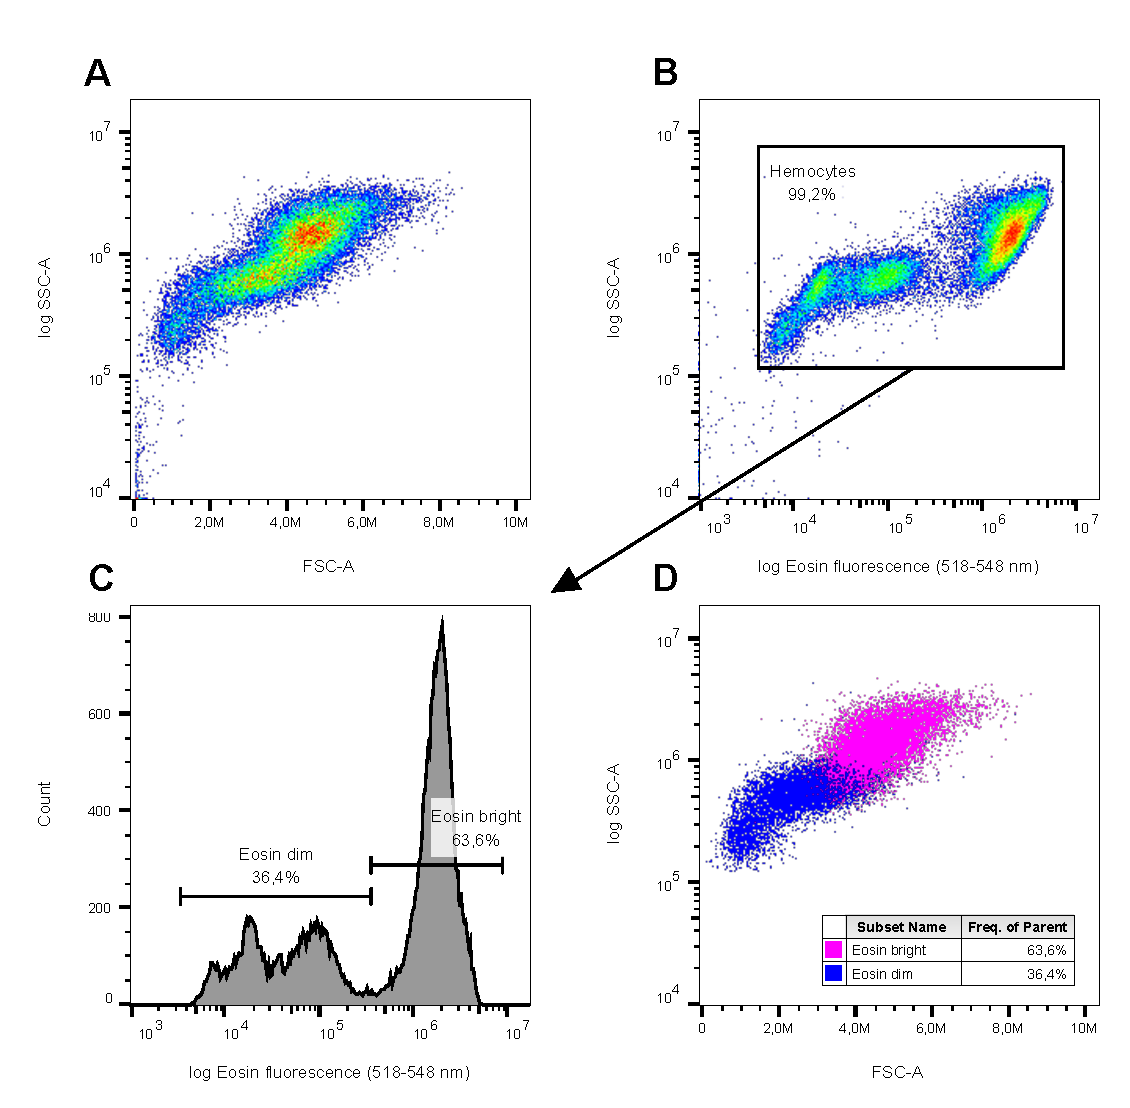
\includegraphics[width=1.0\textwidth]{figures/Eosin and Percoll exp/Eosin exp pool ex for Incskape test.pdf}
    \caption{\textbf{Identification eosinophilic granulocytes by flow cytometry based on eosin fluorescence. A} Representative light scatter profiles of... \textbf{B} }
    \label{fig:eosin_exp}
\end{figure}




\begin{figure}[!ht]
    \centering
    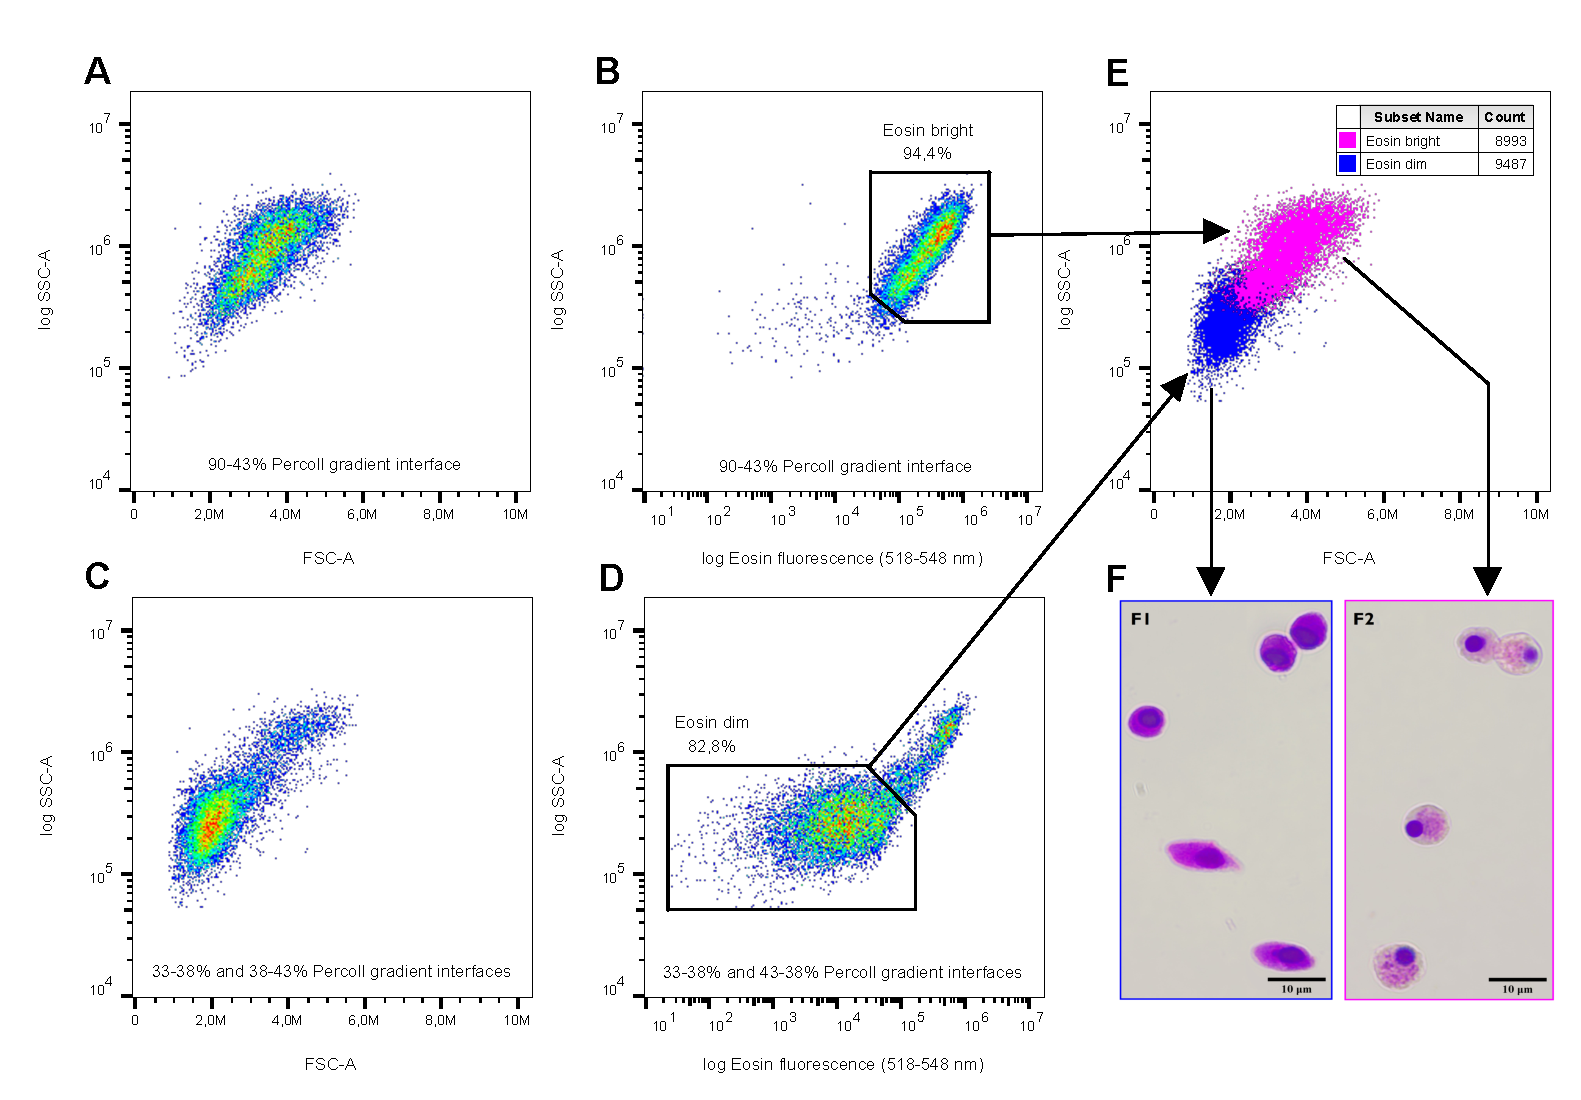
\includegraphics[width=1.0\textwidth]{figures/Eosin and Percoll exp/Percoll sep for Inkscape 2.pdf}
    \caption{\textbf{Confirmation of the light scattering profiles of eosinophilic and basophilic granulocytes pre-separated by discontinuous density centrifugation. A} Light scattering profile of the 95\% pure eosinophilic fraction that separated out on top of the 43-90\% Percoll gradient interface. \textbf{B} Bla bla bla eosin separation bla bla...}
    \label{fig:Percoll-dotplots}
\end{figure}








\chapter{Discussion}
\label{chap:discuss}

This is where you write about your results in the context of what was expected, what others with similar experiments have found (in line with, contradictory, similar to). Put it together with other findings that may be relevant or interesting. The results are interpreted: what do they mean for the field, the risk assessors, the environmental risk of Ti2O, ZnO Ag NPs in the aquatic environment, Trondheimsfjorden. Extrapolate to a greater level of organization?. Put the results into a bigger context.

A small proportion of large cells displayed a strangely similar morphology to the eosinophils, only distinguishable by the fact that their cytoplasm remained unstained with eosin. Whether these cells were a result of staining artifacts or incomplete staining, is not entirely known or easy to determine. Since they fit into the eosinophils according to size and complexity in cluster 3, we assumed them to be incompletely stained eosinophils, and counted them as such when encountered during MN scoring. Discuss this in light of Le Foll et al, 2010 findings, and the fact that we (almost) never encountered them when staining adhered cells according to Bolognesi's MN protocol. Most likely a result of incomplete staining in suspension.

We should have withdrawn two samples from each mussel (as we did), but one into MPSS for staining with the Hemacolor kit and subsequant MN scoring (cold MPSS, 5 min inc in humid chamber) and one into ACB for FCM assays. With a bit dilution in MPSS and short incubation, neither aggregation nor spreading is a problem.

Haemolymph smears can be messy. Therefore, scoring of necrotic and apoptotic haemocytes by microscopy should be performed by certified operators with formal education or practice from hematology or immunology. A few example PNG images with from a published protocol leaves too much to subjectivity. Secondly, if they are rare events (e.g., low dose), why not score all 10 of 100.000 cells objectively by FCM instead of 0 or 1 from 2000 cells in the smear?
\chapter{Conclusion}

You definitely should use the \texttt{ntnuthesis} \LaTeX{} document class for your thesis.



%\newpage
%\chapter{Bibliography}
%\bibliographystyle{unsrtnat}  %Definerer bibliografistil
%{\footnotesize\bibliography{mendeley-entrans.bib, manual-bibtex.bib}}

\chapter*{\bibname}
\printbibliography[heading=none]


\appendix
\chapter{Additional Material}
\label{app:additional}



Additional material that does not fit in the main thesis but may still be relevant to share, e.g., raw data from experiments and surveys, code listings, additional plots, pre-project reports, project agreements, contracts, logs etc., can be put in appendices. Simply issue the command \texttt{\textbackslash appendix} in the main \texttt{.tex} file, and make one chapter per appendix.

If the appendix is in the form of a ready-made PDF file, it should be supported by a small descriptive text, and included using the \texttt{pdfpages} package. To illustrate how it works, a standard project agreement (for the IE faculty at NTNU in Gjøvik) is attached here. You would probably want the included PDF file to begin on an odd (right hand) page, which is achieved by using the \texttt{\textbackslash cleardoublepage} command immediately before the \texttt{\textbackslash includepdf[]\{\}} command. Use the option \texttt{[pages=-]} to include all pages of the PDF document, or, e.g., \texttt{[pages=2-4]} to include only the given page range.
\chapter{Raw data}
\label{app:rawdata}


\section{Method development: raw data}
\subsection{Hemocyte medium proportion aggregation data}

\begin{center}
\begin{longtable}{ccccc}
\caption{The buffer aggregation proportion raw data longtable.}\label{tab:long_table1} \\
\hline
Mussel ID & Buffer & t (min) & $N_{tx}$ & $N_{t0}$ \\
\hline 
\endfirsthead

\multicolumn{5}{c}%
{{\bfseries \tablename\ \thetable{} -- continued from previous page}} \\

\hline
Mussel ID & Buffer & t (min) & $N_{tx}$ & $N_{t0}$ \\ 
\hline 
\endhead

\hline \multicolumn{5}{|r|}{{Continued on next page}} \\ \hline
\endfoot

\hline \hline
\endlastfoot	
M1	&	MAS	&	0.000001	&	36877	&	36877	\\
M1	&	MAS	&	19	&	23728	&	36877	\\
M1	&	MAS	&	49	&	13479	&	36877	\\
M1	&	MAS	&	78	&	5209	&	36877	\\
M2	&	MAS	&	0.000001	&	25544	&	25544	\\
M2	&	MAS	&	15	&	17570	&	25544	\\
M2	&	MAS	&	45	&	8195	&	25544	\\
M2	&	MAS	&	69	&	5060	&	25544	\\
M3	&	MAS	&	0.000001	&	24381	&	24381	\\
M3	&	MAS	&	16	&	21462	&	24381	\\
M3	&	MAS	&	47	&	9347	&	24381	\\
M3	&	MAS	&	67	&	8525	&	24381	\\
M4	&	MAS	&	0.000001	&	27327	&	27327	\\
M4	&	MAS	&	15	&	26100	&	27327	\\
M4	&	MAS	&	30	&	22529	&	27327	\\
M4	&	MAS	&	59	&	8333	&	27327	\\
M5	&	MAS	&	0.000001	&	12889	&	12889	\\
M5	&	MAS	&	15	&	10605	&	12889	\\
M5	&	MAS	&	30	&	8146	&	12889	\\
M5	&	MAS	&	60	&	3450	&	12889	\\
M6	&	MAS	&	0.000001	&	2519	&	2519	\\
M6	&	MAS	&	45	&	2107	&	2519	\\
M6	&	MAS	&	70	&	1627	&	2519	\\
M7	&	MAS	&	0.000001	&	4131	&	4131	\\
M7	&	MAS	&	45	&	2622	&	4131	\\
M7	&	MAS	&	69	&	2149	&	4131	\\
A1	&	ACB	&	0.000001	&	876	&	876	\\
A1	&	ACB	&	19	&	504	&	876	\\
A1	&	ACB	&	37	&	477	&	876	\\
A1	&	ACB	&	67	&	344	&	876	\\
A2	&	ACB	&	0.000001	&	6835	&	6835	\\
A2	&	ACB	&	17	&	5430	&	6835	\\
A2	&	ACB	&	34	&	3411	&	6835	\\
A2	&	ACB	&	64	&	3942	&	6835	\\
A3	&	ACB	&	0.000001	&	14829	&	14829	\\
A3	&	ACB	&	17	&	13764	&	14829	\\
A3	&	ACB	&	32	&	8520	&	14829	\\
A3	&	ACB	&	63	&	4579	&	14829	\\
A4	&	ACB	&	0.000001	&	48859	&	48859	\\
A4	&	ACB	&	15	&	44741	&	48859	\\
A4	&	ACB	&	30	&	31079	&	48859	\\
A4	&	ACB	&	60	&	11281	&	48859	\\
A5	&	ACB	&	0.000001	&	5641	&	5641	\\
A5	&	ACB	&	15	&	3079	&	5641	\\
A5	&	ACB	&	30	&	2466	&	5641	\\
A5	&	ACB	&	45	&	2413	&	5641	\\
A6	&	ACB	&	0.000001	&	10140	&	10140	\\
A6	&	ACB	&	15	&	8912	&	10140	\\
A6	&	ACB	&	30	&	5353	&	10140	\\
A6	&	ACB	&	45	&	3681	&	10140	\\
A7	&	ACB	&	0.000001	&	39534	&	39534	\\
A7	&	ACB	&	17	&	20087	&	39534	\\
A7	&	ACB	&	32	&	14581	&	39534	\\
A7	&	ACB	&	47	&	10109	&	39534	\\
A8	&	ACB	&	0.000001	&	16736	&	16736	\\
A8	&	ACB	&	15	&	11449	&	16736	\\
A8	&	ACB	&	30	&	8935	&	16736	\\
A8	&	ACB	&	45	&	5145	&	16736	\\
H1	&	MPSS	&	0.000001	&	2447	&	2447	\\
H1	&	MPSS	&	15	&	823	&	2447	\\
H1	&	MPSS	&	30	&	887	&	2447	\\
H1	&	MPSS	&	45	&	972	&	2447	\\
H1	&	MPSS	&	60	&	798	&	2447	\\
H2	&	MPSS	&	0.000001	&	2645	&	2645	\\
H2	&	MPSS	&	15	&	1693	&	2645	\\
H2	&	MPSS	&	30	&	1779	&	2645	\\
H2	&	MPSS	&	45	&	1438	&	2645	\\
H2	&	MPSS	&	60	&	1419	&	2645	\\
H3	&	MPSS	&	0.000001	&	2377	&	2377	\\
H3	&	MPSS	&	15	&	1318	&	2377	\\
H3	&	MPSS	&	30	&	1064	&	2377	\\
H3	&	MPSS	&	45	&	862	&	2377	\\
H3	&	MPSS	&	60	&	659	&	2377	\\
H4	&	MPSS	&	0.000001	&	2879	&	2879	\\
H4	&	MPSS	&	15	&	1624	&	2879	\\
H4	&	MPSS	&	30	&	1617	&	2879	\\
H4	&	MPSS	&	45	&	1049	&	2879	\\
H4	&	MPSS	&	60	&	1120	&	2879	\\
H5	&	MPSS	&	0.000001	&	3151	&	3151	\\
H5	&	MPSS	&	15	&	1445	&	3151	\\
H5	&	MPSS	&	30	&	1125	&	3151	\\
H5	&	MPSS	&	45	&	984	&	3151	\\
H5	&	MPSS	&	60	&	414	&	3151	\\
H6	&	MPSS	&	0.000001	&	1699	&	1699	\\
H6	&	MPSS	&	15	&	1080	&	1699	\\
H6	&	MPSS	&	31	&	733	&	1699	\\
H6	&	MPSS	&	45	&	811	&	1699	\\
H6	&	MPSS	&	60	&	715	&	1699	\\
H7	&	MPSS	&	0.000001	&	3309	&	3309	\\
H7	&	MPSS	&	15	&	1634	&	3309	\\
H7	&	MPSS	&	31	&	1453	&	3309	\\
H7	&	MPSS	&	46	&	1415	&	3309	\\
H7	&	MPSS	&	60	&	1393	&	3309	\\
H8	&	MPSS	&	0.000001	&	2822	&	2822	\\
H8	&	MPSS	&	15	&	1460	&	2822	\\
H8	&	MPSS	&	30	&	1518	&	2822	\\
H8	&	MPSS	&	45	&	1475	&	2822	\\
H8	&	MPSS	&	60	&	1346	&	2822	\\
\end{longtable}    
\end{center}

\pagebreak


\subsection{Hemocyte medium viability raw data}

\begin{center}
\begin{longtable}{cccccc}
\caption{The buffer viability raw data longtable.} \label{tab:long_table2} \\
\hline
\multirow{2}{*}{Buffer} & \multirow{2}{*}{Incubation} & \multicolumn{4}{c}{Count} \\
  && CAM$^{+}$ TP3$^{-}$ & CAM$^{+}$ TP3$^{+}$ & CAM$^{-}$TP3$^{+}$ & CAM$^{-}$ TP3$^{-}$ \\ 
\hline 
\endfirsthead

\multicolumn{6}{c}%
{{\bfseries \tablename\ \thetable{} -- continued from previous page}} \\

\hline
\multirow{2}{*}{Buffer} & \multirow{2}{*}{Incubation} & \multicolumn{4}{c}{Count} \\
 && CAM$^{+}$ TP3$^{-}$ & CAM$^{+}$ TP3$^{+}$ & CAM$^{-}$TP3$^{+}$ & CAM$^{-}$ TP3$^{-}$ \\ 
\hline 
\endhead

\hline \multicolumn{6}{|r|}{{Continued on next page}} \\ \hline
\endfoot

\hline \hline
\endlastfoot
ACB	&	15 min	&	9957	&	1	&	28	&	12	\\
ACB	&	15 min	&	9907	&	12	&	44	&	1	\\
ACB	&	15 min	&	9970	&	1	&	27	&	8	\\
ACB	&	15 min	&	9942	&	8	&	34	&	32	\\
ACB	&	15 min	&	9925	&	7	&	45	&	10	\\
ACB	&	15 min	&	9946	&	5	&	17	&	3	\\
ACB	&	15 min	&	9989	&	1	&	16	&	3	\\
ACB	&	15 min	&	9970	&	9	&	23	&	6	\\
MPSS	&	15 min	&	7707	&	3	&	5	&	4	\\
MPSS	&	15 min	&	6622	&	3	&	8	&	5	\\
MPSS	&	15 min	&	5748	&	8	&	20	&	3	\\
MPSS	&	15 min	&	10040	&	0	&	30	&	57	\\
MPSS	&	15 min	&	9937	&	1	&	13	&	49	\\
MPSS	&	15 min	&	9929	&	2	&	24	&	45	\\
MPSS	&	15 min	&	9950	&	0	&	32	&	18	\\
MPSS	&	15 min	&	9970	&	2	&	15	&	13	\\
MAS	&	15 min	&	8600	&	1	&	15	&	8	\\
MAS	&	15 min	&	9033	&	0	&	30	&	5	\\
MAS	&	15 min	&	8340	&	1	&	9	&	7	\\
MAS	&	15 min	&	8633	&	0	&	7	&	12	\\
MAS	&	15 min	&	7901	&	2	&	17	&	3	\\
MAS	&	15 min	&	8863	&	0	&	10	&	1	\\
MAS	&	15 min	&	9133	&	3	&	17	&	2	\\
MAS	&	15 min	&	8929	&	0	&	12	&	12	\\
ACB	&	2 hours	&	9457	&	4	&	62	&	252	\\
ACB	&	2 hours	&	9792	&	12	&	67	&	70	\\
ACB	&	2 hours	&	9984	&	4	&	58	&	109	\\
ACB	&	2 hours	&	1829	&	0	&	16	&	11	\\
ACB	&	2 hours	&	6801	&	2	&	21	&	237	\\
ACB	&	2 hours	&	4403	&	0	&	17	&	307	\\
ACB	&	2 hours	&	9752	&	5	&	86	&	241	\\
ACB	&	2 hours	&	9875	&	5	&	34	&	123	\\
MPSS	&	2 hours	&	9276	&	21	&	12	&	56	\\
MPSS	&	2 hours	&	6279	&	14	&	2	&	39	\\
MPSS	&	2 hours	&	4869	&	3	&	3	&	43	\\
MPSS	&	2 hours	&	4680	&	13	&	4	&	414	\\
MPSS	&	2 hours	&	6174	&	4	&	0	&	60	\\
MPSS	&	2 hours	&	7573	&	6	&	5	&	37	\\
MPSS	&	2 hours	&	8131	&	25	&	6	&	103	\\
MPSS	&	2 hours	&	8930	&	10	&	0	&	93	\\
MAS	&	2 hours	&	5061	&	0	&	28	&	64	\\
MAS	&	2 hours	&	4947	&	2	&	39	&	103	\\
MAS	&	2 hours	&	9973	&	11	&	62	&	58	\\
MAS	&	2 hours	&	6190	&	8	&	14	&	74	\\
MAS	&	2 hours	&	8473	&	0	&	21	&	104	\\
MAS	&	2 hours	&	9884	&	8	&	64	&	118	\\
MAS	&	2 hours	&	9930	&	5	&	22	&	124	\\
MAS	&	2 hours	&	9953	&	0	&	28	&	19	\\
ACB	&	20 hours	&	9135	&	8	&	541	&	206	\\
ACB	&	20 hours	&	7519	&	1	&	1559	&	341	\\
ACB	&	20 hours	&	7383	&	4	&	994	&	594	\\
ACB	&	20 hours	&	9668	&	7	&	340	&	285	\\
ACB	&	20 hours	&	10054	&	2	&	143	&	134	\\
ACB	&	20 hours	&	9103	&	27	&	637	&	118	\\
ACB	&	20 hours	&	8198	&	4	&	896	&	234	\\
ACB	&	20 hours	&	8174	&	2	&	969	&	328	\\
MPSS	&	20 hours	&	9577	&	29	&	51	&	7	\\
MPSS	&	20 hours	&	9277	&	11	&	371	&	33	\\
MPSS	&	20 hours	&	9651	&	12	&	41	&	11	\\
MPSS	&	20 hours	&	9355	&	22	&	149	&	12	\\
MPSS	&	20 hours	&	9879	&	9	&	59	&	23	\\
MPSS	&	20 hours	&	9736	&	89	&	69	&	56	\\
MPSS	&	20 hours	&	9933	&	2	&	18	&	8	\\
MPSS	&	20 hours	&	9693	&	6	&	158	&	32	\\
MAS	&	20 hours	&	8025	&	24	&	523	&	578	\\
MAS	&	20 hours	&	8910	&	3	&	382	&	210	\\
MAS	&	20 hours	&	8502	&	1	&	453	&	523	\\
MAS	&	20 hours	&	9663	&	4	&	370	&	417	\\
MAS	&	20 hours	&	8959	&	16	&	1088	&	607	\\
MAS	&	20 hours	&	9640	&	3	&	446	&	467	\\
MAS	&	20 hours	&	8537	&	6	&	675	&	309	\\
MAS	&	20 hours	&	9237	&	10	&	1033	&	685	\\

\end{longtable}    
\end{center}

\subsection{Experimental determination of optimal TO-PRO-3 Iodide concentration}

The raw data from the experimental determination of an optimal TO-PRO$^{TM}$-3 Iodide concentration for a flow cytometric dye exclusion test is shown in table \ref{tb:ToPro3_stainopt}. The estimated parameters of the fitted log-logistic model are presented in \ref{tb:loglogistic_ToPro3}.


\begin{table}[H]
	\centering
	\caption{Raw data from the experimental determination of the optimal range of TO-PRO$^{TM}$-3 Iodide concentrations for a flow cytometric dye exclusion test of membrane integrity. The table lists the TO-PRO$^{TM}$-3 concentrations tested (\micro M),  incubation durations (min), the mean fluorescent intensity (MFI) of viable (ToPro$^{-}$) and \ce{MeOH}-killed haemocytes (ToPro$^{+}$) and the difference between the two (MFI$_{ToPro3^{+}}$ - MFI$_{ToPro3^{-}}$). Samples were analyzed on a BD Accuri C6 Plus flow cytometer (BD Biosciences, California, US) and MFI's were calculated using FlowJo$^{TM}$ v10.8 Software (BD Life Sciences).}
	\label{tb:ToPro3_stainopt}
	\resizebox{\linewidth}{!}{
	\begin{tabular}{ccccc}
        \toprule
	    \multirow{2}[-5]{*}{TO-PRO$^{TM}$-3 Iodide} & \multirow{2}[-5]{*}{Incubation} & \multicolumn{2}{c}{Mean Fluorescent Intensity} & \multirow{2}{*}{MFI$_{ToPro3^{+}}$ - MFI$_{ToPro3^{-}}$} \\
        (\micro M) & (min) & ToPro3$^{+}$ & ToPro3$^{-}$ & \\
		\midrule
  0     &   15  &    764    &   554     &   210 \\
0.03	&	15	&	867000	&	6750	&	860250	\\
0.06	&	15	&	865000	&	6488	&	858512	\\
0.1	&	15	&	2670000	&	19378	&	2650622	\\
0.3	&	15	&	3710000	&	43720	&	3666280	\\
0.2	&	15	&	3750000	&	41441	&	3708559	\\
0.6	&	15	&	5920000	&	62519	&	5857481	\\
0.6	&	15	&	5330000	&	40903	&	5289097	\\
1.2	&	15	&	7700000	&	103179	&	7596821	\\
2	&	15	&	8550000	&	298543	&	8251457	\\
4	&	15	&	9240000	&	352373	&	8887627	\\
8	&	15	&	9550000	&	456001	&	9093999	\\
0.1	&	30	&	2470000	&	28374	&	2441626	\\
0.2	&	30	&	3860000	&	48720	&	3811280	\\
0.3	&	30	&	3640000	&	68309	&	3571691	\\
0.6	&	30	&	5690000	&	94568	&	5595432	\\
0.6	&	30	&	5320000	&	60620	&	5259380	\\
1.2	&	30	&	7580000	&	155710	&	7424290	\\
2	&	30	&	8710000	&	486028	&	8223972	\\
4	&	30	&	9410000	&	577181	&	8832819	\\
8	&	30	&	9670000	&	713160	&	8956840	\\
   		\bottomrule
	\end{tabular}
}
\end{table}


\begin{table}[H]
	\centering
	\caption{Log-logistic regression analysis of the relationship between TO-PRO$^{TM}$-3 Iodide concentration and the difference in median fluorescent intensity (MFI) between ToPro3$^{-}$ and ToPro3$^{-}$ populations. Parameter estimates with 95\% CI, standard errors, t-value and the belonging p-value.}
	\label{tb:loglogistic_ToPro3}
	\resizebox{\linewidth}{!}{
	\begin{tabular}{cccccc}
        \toprule
	\textbf{Parameter} & \textbf{Estimate} & \textbf{95\% CI} & \textbf{Std. Error} & \textbf{t-value} & \textbf{Pr(T > $\mid$ t $\mid)$} \\
		\midrule
  \emph{b} & -0.94088 & [-1.182762, -0.6989903] & 0.11 & -8.7992 & < 0.001 \\
  \emph{d} & 9890700  & [8701569, 11079860]     & 530000 & 18.8155 & < 0.001 \\
  \emph{e} & 0.41655  & [0.2622887, 0.5708113]  & 0.068 & 6.10085 & < 0.001 \\
  &&&&& \\
  \multicolumn{6}{l}{Pseudo R$^{2}$ = 0.99} \\
  \multicolumn{6}{l}{Residual standard error: 416074.3 on 9 degrees of freedom} \\
		\bottomrule
	\end{tabular}
	}
\end{table}



Pseudo-R$^{2}$ by (\cite{Shabenberger2002}), which the statistic used by the \emph{R2nls} function for .nls and .drm type objects in the \emph{aomisc} package in R.

\begin{equation}
\label{eq:PseudoR2}
Pseudo ~ R^2 = 1 - \dfrac{SS_{res}}{SS_{tot}}
\end{equation}



\end{document}
